\clearpage
\section*{Задание второго этапа}
\phantomsection
\addcontentsline{toc}{section}{Задание второго этапа}

Второй этап курсовой работы включает:

\begin{enumerate}
\item Построение ER-модели не менее чем с 10 сущностями и связью «многие ко многим».
\item Построение даталогической модели на основе ER-модели.
\item Реализацию модели в Postgre\allowbreak{}SQL.
\item Обеспечение целостности средствами DDL и триггеров.
\item Скрипты создания, удаления и заполнения тестовыми данными.
\item Функции и процедуры PL/\allowbreak{}pg\allowbreak{}SQL для критически важных запросов.
\item Индексы по прецедентам первого этапа и обоснование их полезности.
\item Подготовку отчёта.
\end{enumerate}

\clearpage
\section{ER-модель базы данных}

\FloatBarrier
\Needspace{6\baselineskip}
\subsection{Сущности и связи}

Модель построена по процессам и прецедентам первого этапа и содержит 27 сущностей: пользователи, роли, назначения ролей, проверки профилей, одноразовые токены, токены обновления, тарифы, заказы оплаты, платёжные события, периоды подписки, организации, места, категории, объявления, изображения, контрольные признаки, заявки на передачу, диалоги, сообщения, передачи, жалобы, допуски к продаже, аукционы, ставки, уведомления, события доставки и записи аудита.

Пользователь может иметь несколько ролей, а одна роль назначается нескольким пользователям. Отношение «многие ко многим» реализовано ассоциативной сущностью «Назначение роли»: lf\_\allowbreak{}user\_\allowbreak{}roles(user\_\allowbreak{}id, role\_\allowbreak{}code). Составной первичный ключ исключает повторное назначение одной роли пользователю.

Объявление принадлежит одному автору, одной категории и одному месту. Место может быть связано с организацией, предоставляющей справочную информацию. Организация-хранитель находки задаётся отдельно: событие могло произойти в одном месте, а вещь передана другой организации. Поле custodian\_\allowbreak{}org\_\allowbreak{}id не означает партнёрство организации с приложением.

Заявка связывает находку с претендентом. У находки может быть несколько заявок, но один действующий резерв. Диалог и передача относятся к конкретной заявке; участники определяются через автора объявления и заявителя. Необязательный auction\_\allowbreak{}id с внешним ключом и UNIQUE связывает дело передачи с завершённым аукционом: одному аукциону соответствует не более одного такого дела. Допуск к продаже относится к находке и продавцу; каждый аукцион использует конкретный допуск. Это исключает подстановку разрешения для другой вещи. Всего модель содержит 42 внешних ключа.

Заказ оплаты фиксирует стоимость и длительность тарифа на момент создания. Изменение справочника тарифов не меняет уже созданный заказ. Внешние события оплаты отделены от периодов подписки, поскольку платёжный сервис может повторить событие. Одному оплаченному заказу соответствует не более одного периода.

Уведомление адресовано пользователю. Событие доставки содержит тип агрегата, его идентификатор и JSON-параметры; эта техническая очередь не имеет универсального внешнего ключа на разные таблицы. Аудит хранит таблицу и идентификатор изменённой сущности. Его actor\_\allowbreak{}id может быть NULL для фоновой операции.

\FloatBarrier
\Needspace{6\baselineskip}
\subsection{Диаграммы}

Модель разделена на шесть листов для чтения в формате A4. Листы показывают основные связи и их мощности; повтор сущности на разных листах не означает дополнительную таблицу. Полный перечень внешних ключей и атрибутов приведён в даталогической модели и словаре отношений. Обозначения: 1 — ровно один, 0..1 — необязательный экземпляр, 0..N — множество.

\FloatBarrier
\begin{figure}[htbp]
\centering
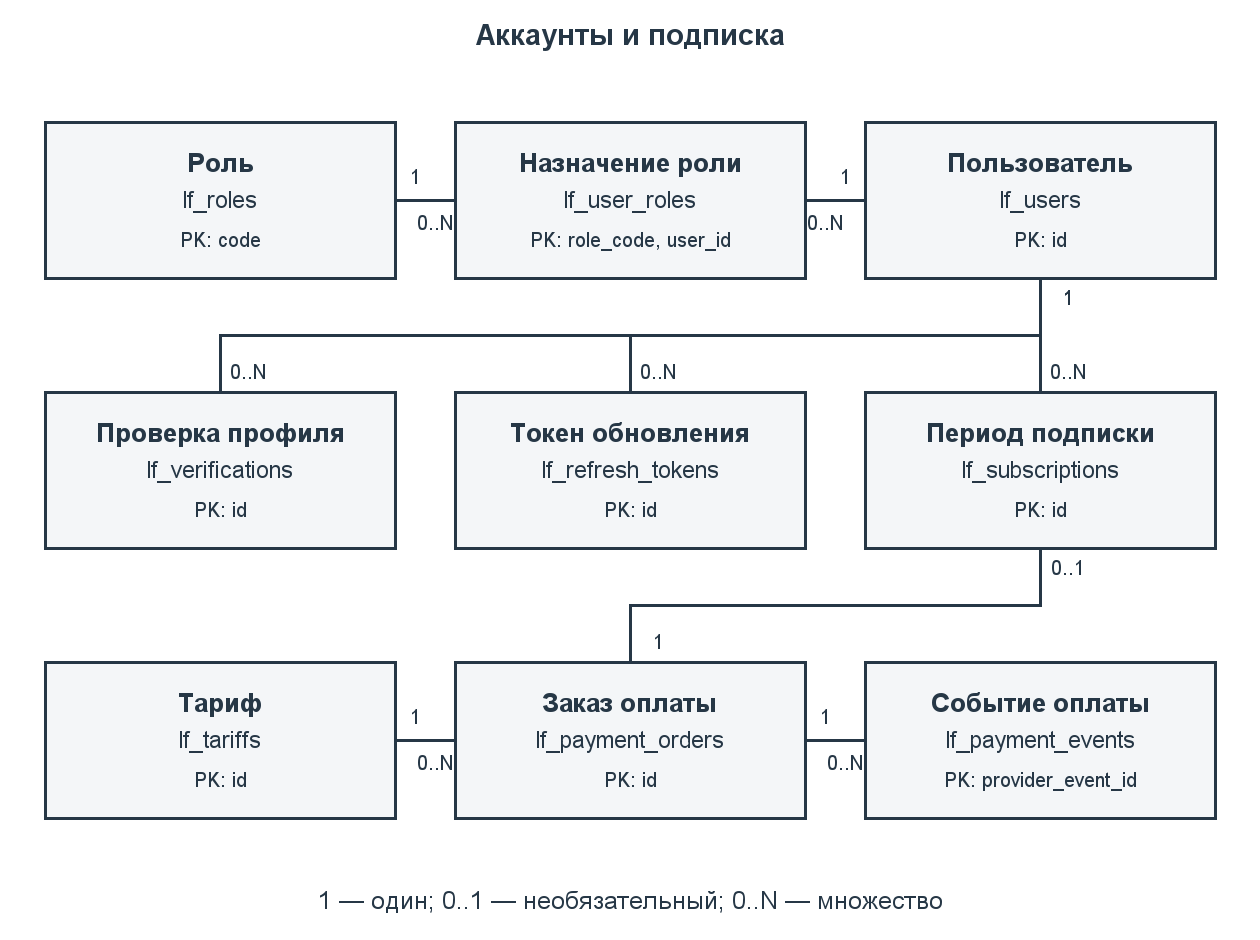
\includegraphics[width=\linewidth,height=0.82\textheight,keepaspectratio]{model/01_accounts.png}
\caption*{Рисунок 7 — ER-модель: аккаунты и подписка}
\end{figure}
\FloatBarrier

\FloatBarrier
\begin{figure}[htbp]
\centering
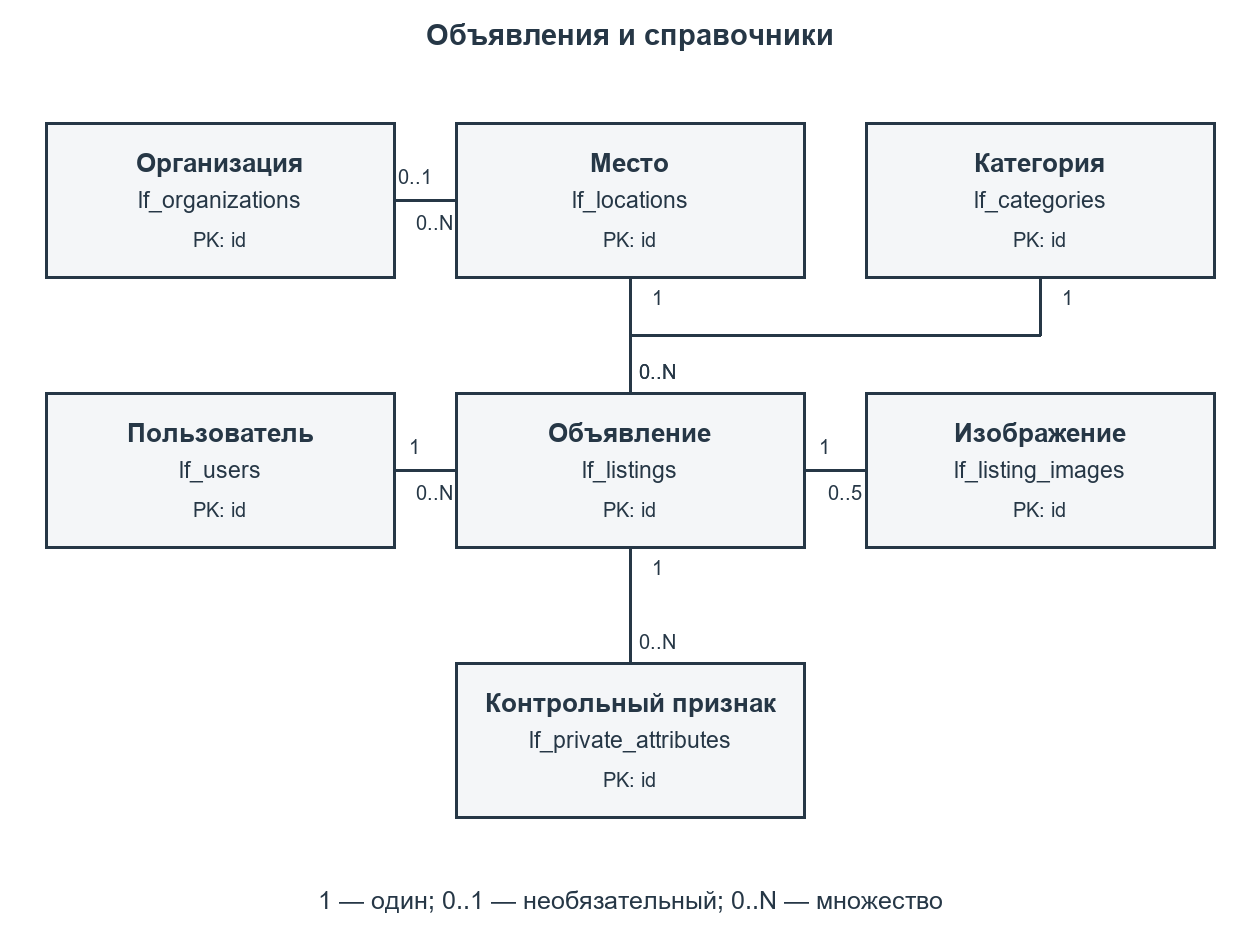
\includegraphics[width=\linewidth,height=0.82\textheight,keepaspectratio]{model/02_listings.png}
\caption*{Рисунок 8 — ER-модель: объявления и справочники}
\end{figure}
\FloatBarrier

\FloatBarrier
\begin{figure}[htbp]
\centering
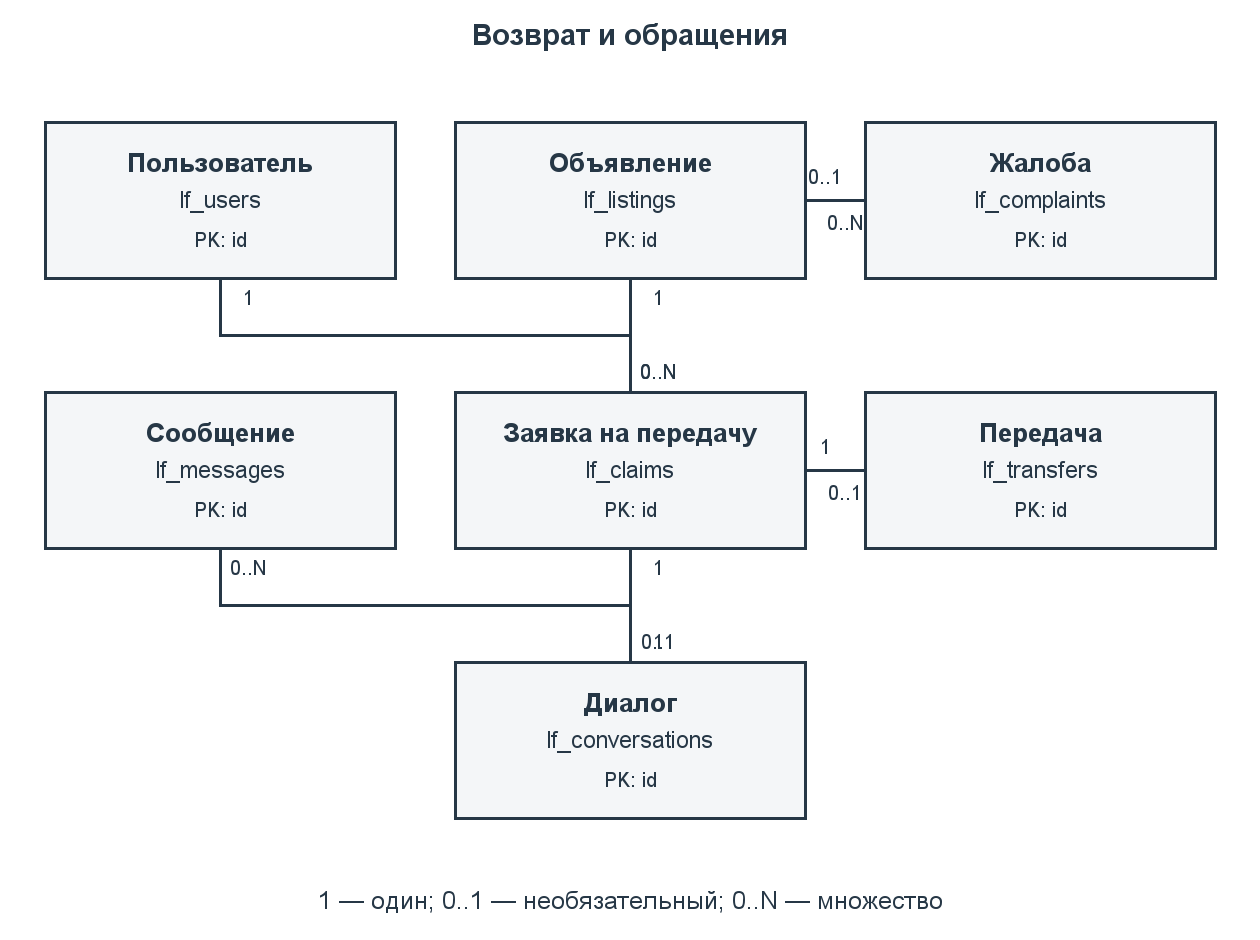
\includegraphics[width=\linewidth,height=0.82\textheight,keepaspectratio]{model/03_returns.png}
\caption*{Рисунок 9 — ER-модель: возврат и обращения}
\end{figure}
\FloatBarrier

\FloatBarrier
\begin{figure}[htbp]
\centering
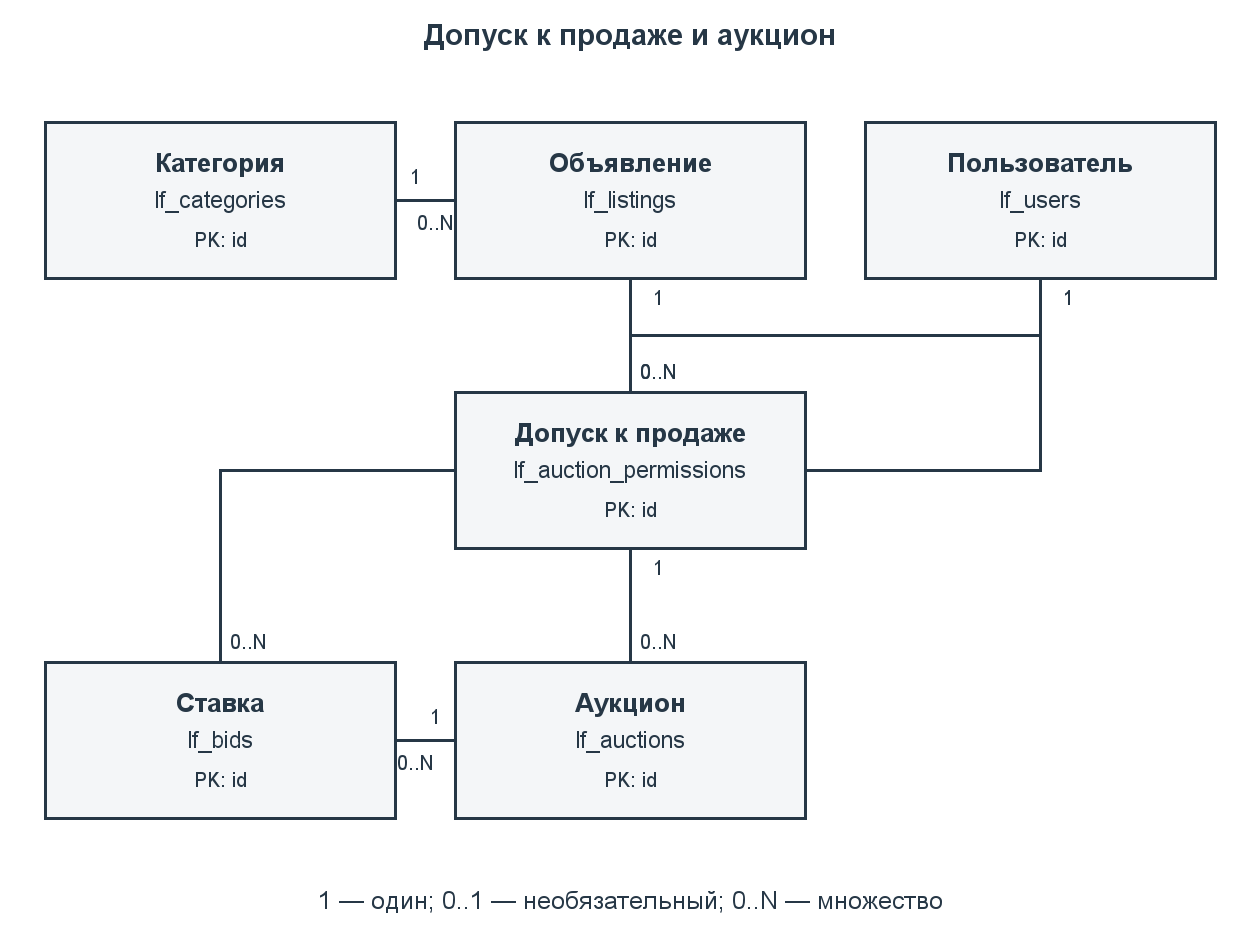
\includegraphics[width=\linewidth,height=0.82\textheight,keepaspectratio]{model/04_auctions.png}
\caption*{Рисунок 10 — ER-модель: аукционы}
\end{figure}
\FloatBarrier

\FloatBarrier
\begin{figure}[htbp]
\centering
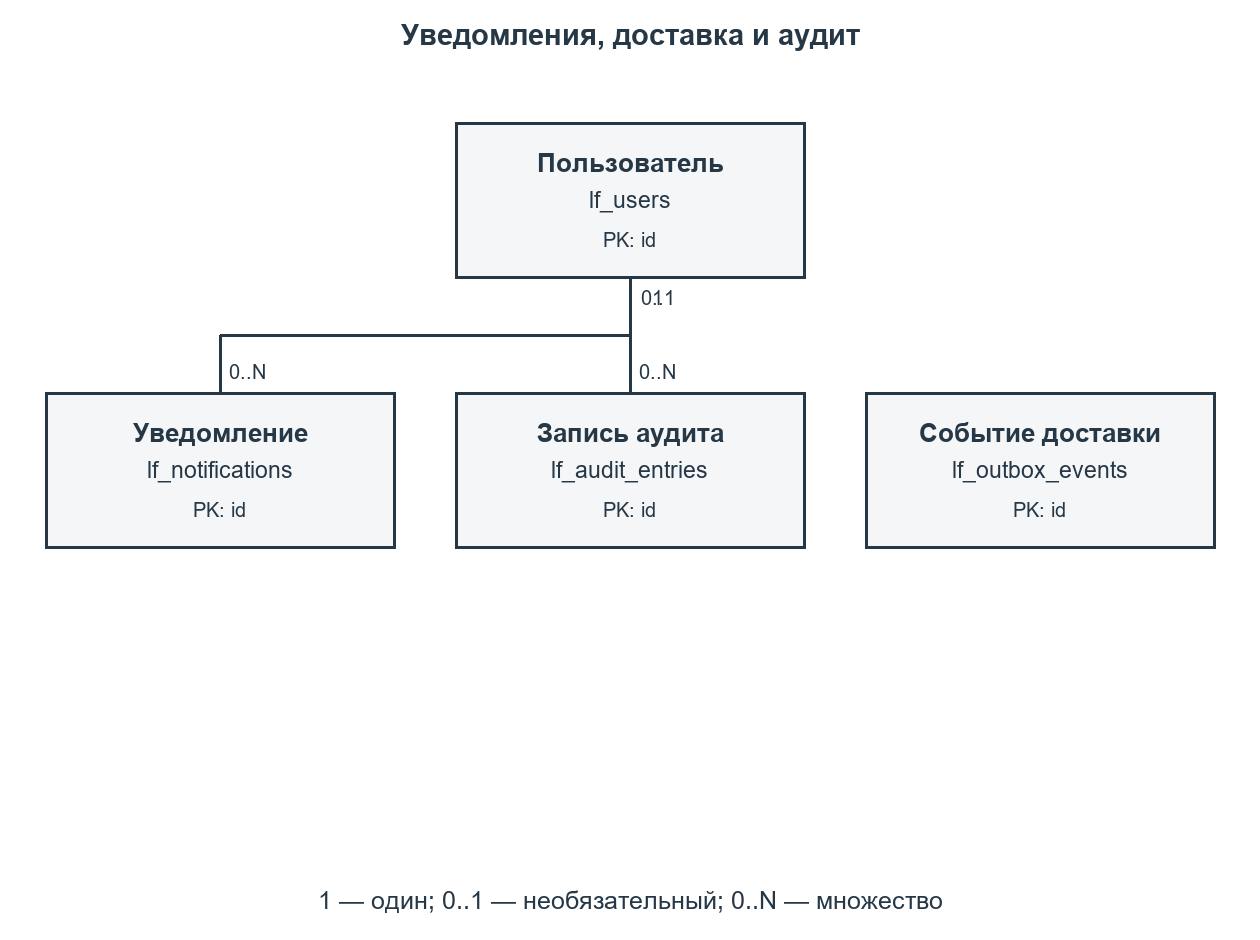
\includegraphics[width=\linewidth,height=0.82\textheight,keepaspectratio]{model/05_events.png}
\caption*{Рисунок 11 — ER-модель: уведомления, доставка и аудит}
\end{figure}
\FloatBarrier

\FloatBarrier
\begin{figure}[htbp]
\centering
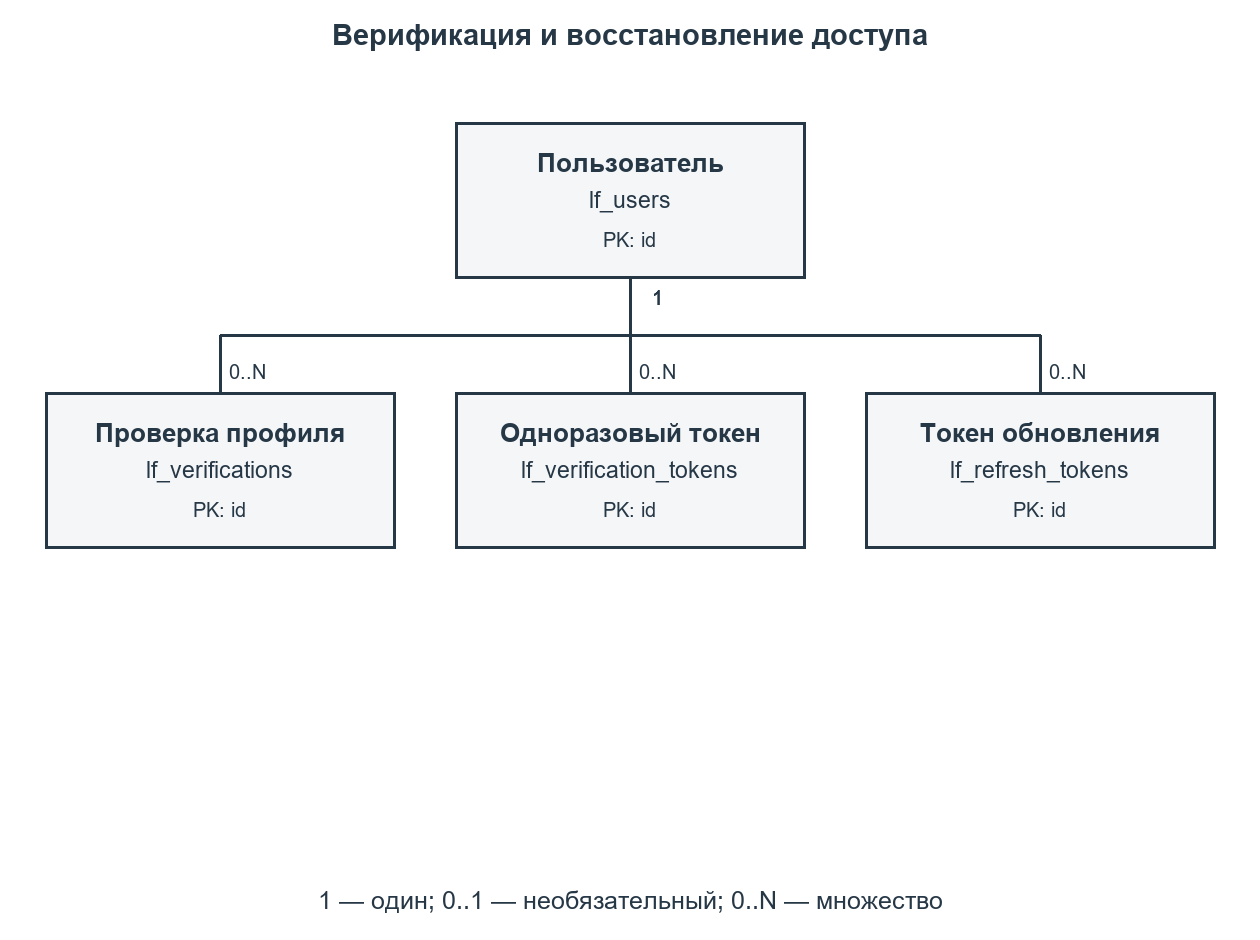
\includegraphics[width=\linewidth,height=0.82\textheight,keepaspectratio]{model/06_tokens.png}
\caption*{Рисунок 12 — ER-модель: верификация и токены}
\end{figure}
\FloatBarrier

Редактируемая концептуальная модель находится в docs/\allowbreak{}part2/\allowbreak{}model/\allowbreak{}er.mmd, полная даталогическая схема — в logical.mmd. Формат Mermaid поддерживает отображение ER-диаграмм и связей с ключами. Изображения каждого листа предоставлены в PNG и SVG.

\clearpage
\section{Даталогическая модель}

\FloatBarrier
\Needspace{6\baselineskip}
\subsection{Преобразование ER-модели}

Каждая сущность преобразована в таблицу Postgre\allowbreak{}SQL. Основные идентификаторы — bigint GENERATED BY DEFAULT AS IDENTITY; код роли является естественным ключом. Для ассоциации пользователей и ролей выбран составной ключ. Связи 1:N реализованы внешними ключами; для связей 1:0..1 добавлено UNIQUE: заявка — диалог, заявка — передача и заказ оплаты — период подписки.

Модель приведена к третьей нормальной форме. Атрибуты пользователя не копируются в объявления, диалоги и ставки. Сведения о категории, месте, организации и тарифе вынесены в справочники. Составной ключ назначения роли не содержит атрибутов, зависящих только от одной его части. Снимок суммы и длительности в заказе относится к самому заказу и необходим для сохранения условий оплаты, поэтому не заменяется ссылкой на текущие значения тарифа.

Время хранится в timestamptz. Начало события обязательно; event\_\allowbreak{}until задаётся только для интервала потери. Денежные значения используют numeric(12,2), без float. Закрытые признаки хранятся в lf\_\allowbreak{}private\_\allowbreak{}attributes и отсутствуют в публичном представлении. Файлы представлены ключами вложений закрытого локального каталога; бинарные данные не записываются в Postgre\allowbreak{}SQL. Технические JSON-поля применяются только в очереди событий и аудите, а связи предметной области остаются реляционными.

Циклическая связь аукциона и выигравшей ставки реализована составным внешним ключом (id, winner\_\allowbreak{}bid\_\allowbreak{}id) \ensuremath{\rightarrow} lf\_\allowbreak{}bids(auction\_\allowbreak{}id, id), отложенным до завершения транзакции. Победитель не может относиться к другому аукциону. Отложенная проверка резерва позволяет в одной транзакции согласовать заявку и изменить статус объявления. Физический столбец search\_\allowbreak{}vector является контролируемой избыточностью для поиска: Postgre\allowbreak{}SQL вычисляет его из текста объявления автоматически; в концептуальной нормализованной модели этот атрибут не требуется.

Словарь отношений сформирован из системного каталога Postgre\allowbreak{}SQL после установки на helios. Он отражает реально созданные типы, возможность NULL, первичные и внешние ключи. Отдельные частичные уникальные индексы описаны в разделе 13.

\FloatBarrier
\Needspace{6\baselineskip}
\subsection{Словарь отношений}

\FloatBarrier
\Needspace{6\baselineskip}
\subsubsection*{1. Допуск к продаже: lf\_\allowbreak{}auction\_\allowbreak{}permissions}

\begingroup
\setstretch{1}
\fontsize{11}{13}\selectfont
\setlength{\tablecontentwidth}{\dimexpr\linewidth-8\tabcolsep-5\arrayrulewidth\relax}
\begin{longtable}{|>{\RaggedRight\arraybackslash}p{0.38\tablecontentwidth}|>{\RaggedRight\arraybackslash}p{0.36\tablecontentwidth}|>{\RaggedRight\arraybackslash}p{0.11\tablecontentwidth}|>{\RaggedRight\arraybackslash}p{0.15\tablecontentwidth}|}
\hline
\textbf{Поле} & \textbf{Тип Postgre\allowbreak{}SQL} & \textbf{NULL} & \textbf{Ключ} \\ \hline
\endfirsthead
\textbf{Поле} & \textbf{Тип Postgre\allowbreak{}SQL} & \textbf{NULL} & \textbf{Ключ} \\ \hline
\endhead
\multicolumn{4}{r}{\footnotesize Продолжение на следующей странице} \\
\endfoot
\endlastfoot
id & bigint & Нет & PK \\ \hline
listing\_\allowbreak{}id & bigint & Нет & FK \\ \hline
applicant\_\allowbreak{}id & bigint & Нет & FK \\ \hline
basis & varchar(20) & Нет & — \\ \hline
evidence\_\allowbreak{}object\_\allowbreak{}key & varchar(240) & Нет & — \\ \hline
state & varchar(12) & Нет & — \\ \hline
moderator\_\allowbreak{}id & bigint & Да & FK \\ \hline
reviewed\_\allowbreak{}at & timestamptz & Да & — \\ \hline
reason & text & Да & — \\ \hline
created\_\allowbreak{}at & timestamptz & Нет & — \\ \hline
\end{longtable}
\endgroup

FOREIGN KEY (applicant\_\allowbreak{}id) REFERENCES lf\_\allowbreak{}users(id).

UNIQUE (id, listing\_\allowbreak{}id, applicant\_\allowbreak{}id).

FOREIGN KEY (listing\_\allowbreak{}id) REFERENCES lf\_\allowbreak{}listings(id).

FOREIGN KEY (moderator\_\allowbreak{}id) REFERENCES lf\_\allowbreak{}users(id).

PRIMARY KEY (id).

\FloatBarrier
\Needspace{6\baselineskip}
\subsubsection*{2. Аукцион: lf\_\allowbreak{}auctions}

\begingroup
\setstretch{1}
\fontsize{11}{13}\selectfont
\setlength{\tablecontentwidth}{\dimexpr\linewidth-8\tabcolsep-5\arrayrulewidth\relax}
\begin{longtable}{|>{\RaggedRight\arraybackslash}p{0.38\tablecontentwidth}|>{\RaggedRight\arraybackslash}p{0.36\tablecontentwidth}|>{\RaggedRight\arraybackslash}p{0.11\tablecontentwidth}|>{\RaggedRight\arraybackslash}p{0.15\tablecontentwidth}|}
\hline
\textbf{Поле} & \textbf{Тип Postgre\allowbreak{}SQL} & \textbf{NULL} & \textbf{Ключ} \\ \hline
\endfirsthead
\textbf{Поле} & \textbf{Тип Postgre\allowbreak{}SQL} & \textbf{NULL} & \textbf{Ключ} \\ \hline
\endhead
\multicolumn{4}{r}{\footnotesize Продолжение на следующей странице} \\
\endfoot
\endlastfoot
id & bigint & Нет & PK, FK \\ \hline
listing\_\allowbreak{}id & bigint & Нет & FK \\ \hline
seller\_\allowbreak{}id & bigint & Нет & FK \\ \hline
permission\_\allowbreak{}id & bigint & Нет & FK \\ \hline
starts\_\allowbreak{}at & timestamptz & Нет & — \\ \hline
ends\_\allowbreak{}at & timestamptz & Нет & — \\ \hline
start\_\allowbreak{}price & numeric(12,2) & Нет & — \\ \hline
bid\_\allowbreak{}step & numeric(12,2) & Нет & — \\ \hline
state & varchar(12) & Нет & — \\ \hline
winner\_\allowbreak{}bid\_\allowbreak{}id & bigint & Да & FK \\ \hline
closed\_\allowbreak{}at & timestamptz & Да & — \\ \hline
\end{longtable}
\endgroup

FOREIGN KEY (listing\_\allowbreak{}id) REFERENCES lf\_\allowbreak{}listings(id).

FOREIGN KEY (permission\_\allowbreak{}id, listing\_\allowbreak{}id, seller\_\allowbreak{}id) REFERENCES lf\_\allowbreak{}auction\_\allowbreak{}permissions(id, listing\_\allowbreak{}id, applicant\_\allowbreak{}id).

PRIMARY KEY (id).

FOREIGN KEY (seller\_\allowbreak{}id) REFERENCES lf\_\allowbreak{}users(id).

FOREIGN KEY (id, winner\_\allowbreak{}bid\_\allowbreak{}id) REFERENCES lf\_\allowbreak{}bids(auction\_\allowbreak{}id, id) DEFERRABLE INITIALLY DEFERRED.

\FloatBarrier
\Needspace{6\baselineskip}
\subsubsection*{3. Запись аудита: lf\_\allowbreak{}audit\_\allowbreak{}entries}

\begingroup
\setstretch{1}
\fontsize{11}{13}\selectfont
\setlength{\tablecontentwidth}{\dimexpr\linewidth-8\tabcolsep-5\arrayrulewidth\relax}
\begin{longtable}{|>{\RaggedRight\arraybackslash}p{0.38\tablecontentwidth}|>{\RaggedRight\arraybackslash}p{0.36\tablecontentwidth}|>{\RaggedRight\arraybackslash}p{0.11\tablecontentwidth}|>{\RaggedRight\arraybackslash}p{0.15\tablecontentwidth}|}
\hline
\textbf{Поле} & \textbf{Тип Postgre\allowbreak{}SQL} & \textbf{NULL} & \textbf{Ключ} \\ \hline
\endfirsthead
\textbf{Поле} & \textbf{Тип Postgre\allowbreak{}SQL} & \textbf{NULL} & \textbf{Ключ} \\ \hline
\endhead
\multicolumn{4}{r}{\footnotesize Продолжение на следующей странице} \\
\endfoot
\endlastfoot
id & bigint & Нет & PK \\ \hline
actor\_\allowbreak{}id & bigint & Да & FK \\ \hline
action & varchar(80) & Нет & — \\ \hline
entity\_\allowbreak{}table & varchar(80) & Нет & — \\ \hline
entity\_\allowbreak{}id & bigint & Нет & — \\ \hline
details & jsonb & Нет & — \\ \hline
created\_\allowbreak{}at & timestamptz & Нет & — \\ \hline
\end{longtable}
\endgroup

FOREIGN KEY (actor\_\allowbreak{}id) REFERENCES lf\_\allowbreak{}users(id).

PRIMARY KEY (id).

\FloatBarrier
\Needspace{6\baselineskip}
\subsubsection*{4. Ставка: lf\_\allowbreak{}bids}

\begingroup
\setstretch{1}
\fontsize{11}{13}\selectfont
\setlength{\tablecontentwidth}{\dimexpr\linewidth-8\tabcolsep-5\arrayrulewidth\relax}
\begin{longtable}{|>{\RaggedRight\arraybackslash}p{0.38\tablecontentwidth}|>{\RaggedRight\arraybackslash}p{0.36\tablecontentwidth}|>{\RaggedRight\arraybackslash}p{0.11\tablecontentwidth}|>{\RaggedRight\arraybackslash}p{0.15\tablecontentwidth}|}
\hline
\textbf{Поле} & \textbf{Тип Postgre\allowbreak{}SQL} & \textbf{NULL} & \textbf{Ключ} \\ \hline
\endfirsthead
\textbf{Поле} & \textbf{Тип Postgre\allowbreak{}SQL} & \textbf{NULL} & \textbf{Ключ} \\ \hline
\endhead
\multicolumn{4}{r}{\footnotesize Продолжение на следующей странице} \\
\endfoot
\endlastfoot
id & bigint & Нет & PK \\ \hline
auction\_\allowbreak{}id & bigint & Нет & FK \\ \hline
bidder\_\allowbreak{}id & bigint & Нет & FK \\ \hline
request\_\allowbreak{}key & uuid & Нет & — \\ \hline
amount & numeric(12,2) & Нет & — \\ \hline
placed\_\allowbreak{}at & timestamptz & Нет & — \\ \hline
\end{longtable}
\endgroup

FOREIGN KEY (auction\_\allowbreak{}id) REFERENCES lf\_\allowbreak{}auctions(id).

UNIQUE (auction\_\allowbreak{}id, id).

FOREIGN KEY (bidder\_\allowbreak{}id) REFERENCES lf\_\allowbreak{}users(id).

PRIMARY KEY (id).

UNIQUE (request\_\allowbreak{}key).

\FloatBarrier
\Needspace{6\baselineskip}
\subsubsection*{5. Категория: lf\_\allowbreak{}categories}

\begingroup
\setstretch{1}
\fontsize{11}{13}\selectfont
\setlength{\tablecontentwidth}{\dimexpr\linewidth-8\tabcolsep-5\arrayrulewidth\relax}
\begin{longtable}{|>{\RaggedRight\arraybackslash}p{0.38\tablecontentwidth}|>{\RaggedRight\arraybackslash}p{0.36\tablecontentwidth}|>{\RaggedRight\arraybackslash}p{0.11\tablecontentwidth}|>{\RaggedRight\arraybackslash}p{0.15\tablecontentwidth}|}
\hline
\textbf{Поле} & \textbf{Тип Postgre\allowbreak{}SQL} & \textbf{NULL} & \textbf{Ключ} \\ \hline
\endfirsthead
\textbf{Поле} & \textbf{Тип Postgre\allowbreak{}SQL} & \textbf{NULL} & \textbf{Ключ} \\ \hline
\endhead
\multicolumn{4}{r}{\footnotesize Продолжение на следующей странице} \\
\endfoot
\endlastfoot
id & bigint & Нет & PK \\ \hline
name & varchar(80) & Нет & — \\ \hline
auction\_\allowbreak{}allowed & boolean & Нет & — \\ \hline
\end{longtable}
\endgroup

UNIQUE (name).

PRIMARY KEY (id).

\FloatBarrier
\Needspace{6\baselineskip}
\subsubsection*{6. Заявка на передачу: lf\_\allowbreak{}claims}

\begingroup
\setstretch{1}
\fontsize{11}{13}\selectfont
\setlength{\tablecontentwidth}{\dimexpr\linewidth-8\tabcolsep-5\arrayrulewidth\relax}
\begin{longtable}{|>{\RaggedRight\arraybackslash}p{0.38\tablecontentwidth}|>{\RaggedRight\arraybackslash}p{0.36\tablecontentwidth}|>{\RaggedRight\arraybackslash}p{0.11\tablecontentwidth}|>{\RaggedRight\arraybackslash}p{0.15\tablecontentwidth}|}
\hline
\textbf{Поле} & \textbf{Тип Postgre\allowbreak{}SQL} & \textbf{NULL} & \textbf{Ключ} \\ \hline
\endfirsthead
\textbf{Поле} & \textbf{Тип Postgre\allowbreak{}SQL} & \textbf{NULL} & \textbf{Ключ} \\ \hline
\endhead
\multicolumn{4}{r}{\footnotesize Продолжение на следующей странице} \\
\endfoot
\endlastfoot
id & bigint & Нет & PK \\ \hline
listing\_\allowbreak{}id & bigint & Нет & FK \\ \hline
claimant\_\allowbreak{}id & bigint & Нет & FK \\ \hline
evidence & text & Нет & — \\ \hline
state & varchar(12) & Нет & — \\ \hline
created\_\allowbreak{}at & timestamptz & Нет & — \\ \hline
auction\_\allowbreak{}id & bigint & Да & FK \\ \hline
\end{longtable}
\endgroup

FOREIGN KEY (auction\_\allowbreak{}id) REFERENCES lf\_\allowbreak{}auctions(id).

UNIQUE (auction\_\allowbreak{}id).

FOREIGN KEY (claimant\_\allowbreak{}id) REFERENCES lf\_\allowbreak{}users(id).

UNIQUE (id, listing\_\allowbreak{}id).

FOREIGN KEY (listing\_\allowbreak{}id) REFERENCES lf\_\allowbreak{}listings(id).

PRIMARY KEY (id).

\FloatBarrier
\Needspace{6\baselineskip}
\subsubsection*{7. Жалоба: lf\_\allowbreak{}complaints}

\begingroup
\setstretch{1}
\fontsize{11}{13}\selectfont
\setlength{\tablecontentwidth}{\dimexpr\linewidth-8\tabcolsep-5\arrayrulewidth\relax}
\begin{longtable}{|>{\RaggedRight\arraybackslash}p{0.38\tablecontentwidth}|>{\RaggedRight\arraybackslash}p{0.36\tablecontentwidth}|>{\RaggedRight\arraybackslash}p{0.11\tablecontentwidth}|>{\RaggedRight\arraybackslash}p{0.15\tablecontentwidth}|}
\hline
\textbf{Поле} & \textbf{Тип Postgre\allowbreak{}SQL} & \textbf{NULL} & \textbf{Ключ} \\ \hline
\endfirsthead
\textbf{Поле} & \textbf{Тип Postgre\allowbreak{}SQL} & \textbf{NULL} & \textbf{Ключ} \\ \hline
\endhead
\multicolumn{4}{r}{\footnotesize Продолжение на следующей странице} \\
\endfoot
\endlastfoot
id & bigint & Нет & PK \\ \hline
reporter\_\allowbreak{}id & bigint & Нет & FK \\ \hline
listing\_\allowbreak{}id & bigint & Да & FK \\ \hline
reported\_\allowbreak{}user\_\allowbreak{}id & bigint & Да & FK \\ \hline
reason & text & Нет & — \\ \hline
state & varchar(12) & Нет & — \\ \hline
moderator\_\allowbreak{}id & bigint & Да & FK \\ \hline
resolution & text & Да & — \\ \hline
created\_\allowbreak{}at & timestamptz & Нет & — \\ \hline
\end{longtable}
\endgroup

FOREIGN KEY (listing\_\allowbreak{}id) REFERENCES lf\_\allowbreak{}listings(id).

FOREIGN KEY (moderator\_\allowbreak{}id) REFERENCES lf\_\allowbreak{}users(id).

PRIMARY KEY (id).

FOREIGN KEY (reported\_\allowbreak{}user\_\allowbreak{}id) REFERENCES lf\_\allowbreak{}users(id).

FOREIGN KEY (reporter\_\allowbreak{}id) REFERENCES lf\_\allowbreak{}users(id).

\FloatBarrier
\Needspace{6\baselineskip}
\subsubsection*{8. Диалог: lf\_\allowbreak{}conversations}

\begingroup
\setstretch{1}
\fontsize{11}{13}\selectfont
\setlength{\tablecontentwidth}{\dimexpr\linewidth-8\tabcolsep-5\arrayrulewidth\relax}
\begin{longtable}{|>{\RaggedRight\arraybackslash}p{0.38\tablecontentwidth}|>{\RaggedRight\arraybackslash}p{0.36\tablecontentwidth}|>{\RaggedRight\arraybackslash}p{0.11\tablecontentwidth}|>{\RaggedRight\arraybackslash}p{0.15\tablecontentwidth}|}
\hline
\textbf{Поле} & \textbf{Тип Postgre\allowbreak{}SQL} & \textbf{NULL} & \textbf{Ключ} \\ \hline
\endfirsthead
\textbf{Поле} & \textbf{Тип Postgre\allowbreak{}SQL} & \textbf{NULL} & \textbf{Ключ} \\ \hline
\endhead
\multicolumn{4}{r}{\footnotesize Продолжение на следующей странице} \\
\endfoot
\endlastfoot
id & bigint & Нет & PK \\ \hline
claim\_\allowbreak{}id & bigint & Нет & FK \\ \hline
created\_\allowbreak{}at & timestamptz & Нет & — \\ \hline
\end{longtable}
\endgroup

FOREIGN KEY (claim\_\allowbreak{}id) REFERENCES lf\_\allowbreak{}claims(id).

UNIQUE (claim\_\allowbreak{}id).

PRIMARY KEY (id).

\FloatBarrier
\Needspace{6\baselineskip}
\subsubsection*{9. Изображение: lf\_\allowbreak{}listing\_\allowbreak{}images}

\begingroup
\setstretch{1}
\fontsize{11}{13}\selectfont
\setlength{\tablecontentwidth}{\dimexpr\linewidth-8\tabcolsep-5\arrayrulewidth\relax}
\begin{longtable}{|>{\RaggedRight\arraybackslash}p{0.38\tablecontentwidth}|>{\RaggedRight\arraybackslash}p{0.36\tablecontentwidth}|>{\RaggedRight\arraybackslash}p{0.11\tablecontentwidth}|>{\RaggedRight\arraybackslash}p{0.15\tablecontentwidth}|}
\hline
\textbf{Поле} & \textbf{Тип Postgre\allowbreak{}SQL} & \textbf{NULL} & \textbf{Ключ} \\ \hline
\endfirsthead
\textbf{Поле} & \textbf{Тип Postgre\allowbreak{}SQL} & \textbf{NULL} & \textbf{Ключ} \\ \hline
\endhead
\multicolumn{4}{r}{\footnotesize Продолжение на следующей странице} \\
\endfoot
\endlastfoot
id & bigint & Нет & PK \\ \hline
listing\_\allowbreak{}id & bigint & Нет & FK \\ \hline
object\_\allowbreak{}key & varchar(240) & Нет & — \\ \hline
media\_\allowbreak{}type & varchar(20) & Нет & — \\ \hline
size\_\allowbreak{}bytes & integer & Нет & — \\ \hline
position & smallint & Нет & — \\ \hline
\end{longtable}
\endgroup

FOREIGN KEY (listing\_\allowbreak{}id) REFERENCES lf\_\allowbreak{}listings(id) ON DELETE CASCADE.

UNIQUE (listing\_\allowbreak{}id, "position").

UNIQUE (object\_\allowbreak{}key).

PRIMARY KEY (id).

\FloatBarrier
\Needspace{6\baselineskip}
\subsubsection*{10. Объявление: lf\_\allowbreak{}listings}

\begingroup
\setstretch{1}
\fontsize{11}{13}\selectfont
\setlength{\tablecontentwidth}{\dimexpr\linewidth-8\tabcolsep-5\arrayrulewidth\relax}
\begin{longtable}{|>{\RaggedRight\arraybackslash}p{0.38\tablecontentwidth}|>{\RaggedRight\arraybackslash}p{0.36\tablecontentwidth}|>{\RaggedRight\arraybackslash}p{0.11\tablecontentwidth}|>{\RaggedRight\arraybackslash}p{0.15\tablecontentwidth}|}
\hline
\textbf{Поле} & \textbf{Тип Postgre\allowbreak{}SQL} & \textbf{NULL} & \textbf{Ключ} \\ \hline
\endfirsthead
\textbf{Поле} & \textbf{Тип Postgre\allowbreak{}SQL} & \textbf{NULL} & \textbf{Ключ} \\ \hline
\endhead
\multicolumn{4}{r}{\footnotesize Продолжение на следующей странице} \\
\endfoot
\endlastfoot
id & bigint & Нет & PK \\ \hline
author\_\allowbreak{}id & bigint & Нет & FK \\ \hline
category\_\allowbreak{}id & bigint & Нет & FK \\ \hline
location\_\allowbreak{}id & bigint & Нет & FK \\ \hline
kind & varchar(5) & Нет & — \\ \hline
title & varchar(120) & Нет & — \\ \hline
description & text & Нет & — \\ \hline
event\_\allowbreak{}at & timestamptz & Нет & — \\ \hline
event\_\allowbreak{}until & timestamptz & Да & — \\ \hline
state & varchar(12) & Нет & — \\ \hline
custodian\_\allowbreak{}org\_\allowbreak{}id & bigint & Да & FK \\ \hline
official\_\allowbreak{}reported\_\allowbreak{}at & timestamptz & Да & — \\ \hline
moderator\_\allowbreak{}id & bigint & Да & FK \\ \hline
moderated\_\allowbreak{}at & timestamptz & Да & — \\ \hline
created\_\allowbreak{}at & timestamptz & Нет & — \\ \hline
search\_\allowbreak{}vector & tsvector & Да & — \\ \hline
\end{longtable}
\endgroup

FOREIGN KEY (author\_\allowbreak{}id) REFERENCES lf\_\allowbreak{}users(id).

FOREIGN KEY (category\_\allowbreak{}id) REFERENCES lf\_\allowbreak{}categories(id).

FOREIGN KEY (custodian\_\allowbreak{}org\_\allowbreak{}id) REFERENCES lf\_\allowbreak{}organizations(id).

FOREIGN KEY (location\_\allowbreak{}id) REFERENCES lf\_\allowbreak{}locations(id).

FOREIGN KEY (moderator\_\allowbreak{}id) REFERENCES lf\_\allowbreak{}users(id).

PRIMARY KEY (id).

\FloatBarrier
\Needspace{6\baselineskip}
\subsubsection*{11. Место: lf\_\allowbreak{}locations}

\begingroup
\setstretch{1}
\fontsize{11}{13}\selectfont
\setlength{\tablecontentwidth}{\dimexpr\linewidth-8\tabcolsep-5\arrayrulewidth\relax}
\begin{longtable}{|>{\RaggedRight\arraybackslash}p{0.38\tablecontentwidth}|>{\RaggedRight\arraybackslash}p{0.36\tablecontentwidth}|>{\RaggedRight\arraybackslash}p{0.11\tablecontentwidth}|>{\RaggedRight\arraybackslash}p{0.15\tablecontentwidth}|}
\hline
\textbf{Поле} & \textbf{Тип Postgre\allowbreak{}SQL} & \textbf{NULL} & \textbf{Ключ} \\ \hline
\endfirsthead
\textbf{Поле} & \textbf{Тип Postgre\allowbreak{}SQL} & \textbf{NULL} & \textbf{Ключ} \\ \hline
\endhead
\multicolumn{4}{r}{\footnotesize Продолжение на следующей странице} \\
\endfoot
\endlastfoot
id & bigint & Нет & PK \\ \hline
city & varchar(80) & Нет & — \\ \hline
description & varchar(240) & Нет & — \\ \hline
latitude & numeric(9,6) & Да & — \\ \hline
longitude & numeric(9,6) & Да & — \\ \hline
metro\_\allowbreak{}station & varchar(100) & Да & — \\ \hline
organization\_\allowbreak{}id & bigint & Да & FK \\ \hline
\end{longtable}
\endgroup

FOREIGN KEY (organization\_\allowbreak{}id) REFERENCES lf\_\allowbreak{}organizations(id).

PRIMARY KEY (id).

\FloatBarrier
\Needspace{6\baselineskip}
\subsubsection*{12. Сообщение: lf\_\allowbreak{}messages}

\begingroup
\setstretch{1}
\fontsize{11}{13}\selectfont
\setlength{\tablecontentwidth}{\dimexpr\linewidth-8\tabcolsep-5\arrayrulewidth\relax}
\begin{longtable}{|>{\RaggedRight\arraybackslash}p{0.38\tablecontentwidth}|>{\RaggedRight\arraybackslash}p{0.36\tablecontentwidth}|>{\RaggedRight\arraybackslash}p{0.11\tablecontentwidth}|>{\RaggedRight\arraybackslash}p{0.15\tablecontentwidth}|}
\hline
\textbf{Поле} & \textbf{Тип Postgre\allowbreak{}SQL} & \textbf{NULL} & \textbf{Ключ} \\ \hline
\endfirsthead
\textbf{Поле} & \textbf{Тип Postgre\allowbreak{}SQL} & \textbf{NULL} & \textbf{Ключ} \\ \hline
\endhead
\multicolumn{4}{r}{\footnotesize Продолжение на следующей странице} \\
\endfoot
\endlastfoot
id & bigint & Нет & PK \\ \hline
conversation\_\allowbreak{}id & bigint & Нет & FK \\ \hline
sender\_\allowbreak{}id & bigint & Нет & FK \\ \hline
body & text & Нет & — \\ \hline
sent\_\allowbreak{}at & timestamptz & Нет & — \\ \hline
\end{longtable}
\endgroup

FOREIGN KEY (conversation\_\allowbreak{}id) REFERENCES lf\_\allowbreak{}conversations(id).

PRIMARY KEY (id).

FOREIGN KEY (sender\_\allowbreak{}id) REFERENCES lf\_\allowbreak{}users(id).

\FloatBarrier
\Needspace{6\baselineskip}
\subsubsection*{13. Уведомление: lf\_\allowbreak{}notifications}

\begingroup
\setstretch{1}
\fontsize{11}{13}\selectfont
\setlength{\tablecontentwidth}{\dimexpr\linewidth-8\tabcolsep-5\arrayrulewidth\relax}
\begin{longtable}{|>{\RaggedRight\arraybackslash}p{0.38\tablecontentwidth}|>{\RaggedRight\arraybackslash}p{0.36\tablecontentwidth}|>{\RaggedRight\arraybackslash}p{0.11\tablecontentwidth}|>{\RaggedRight\arraybackslash}p{0.15\tablecontentwidth}|}
\hline
\textbf{Поле} & \textbf{Тип Postgre\allowbreak{}SQL} & \textbf{NULL} & \textbf{Ключ} \\ \hline
\endfirsthead
\textbf{Поле} & \textbf{Тип Postgre\allowbreak{}SQL} & \textbf{NULL} & \textbf{Ключ} \\ \hline
\endhead
\multicolumn{4}{r}{\footnotesize Продолжение на следующей странице} \\
\endfoot
\endlastfoot
id & bigint & Нет & PK \\ \hline
user\_\allowbreak{}id & bigint & Нет & FK \\ \hline
kind & varchar(40) & Нет & — \\ \hline
body & text & Нет & — \\ \hline
read\_\allowbreak{}at & timestamptz & Да & — \\ \hline
created\_\allowbreak{}at & timestamptz & Нет & — \\ \hline
\end{longtable}
\endgroup

PRIMARY KEY (id).

FOREIGN KEY (user\_\allowbreak{}id) REFERENCES lf\_\allowbreak{}users(id).

\FloatBarrier
\Needspace{6\baselineskip}
\subsubsection*{14. Организация: lf\_\allowbreak{}organizations}

\begingroup
\setstretch{1}
\fontsize{11}{13}\selectfont
\setlength{\tablecontentwidth}{\dimexpr\linewidth-8\tabcolsep-5\arrayrulewidth\relax}
\begin{longtable}{|>{\RaggedRight\arraybackslash}p{0.38\tablecontentwidth}|>{\RaggedRight\arraybackslash}p{0.36\tablecontentwidth}|>{\RaggedRight\arraybackslash}p{0.11\tablecontentwidth}|>{\RaggedRight\arraybackslash}p{0.15\tablecontentwidth}|}
\hline
\textbf{Поле} & \textbf{Тип Postgre\allowbreak{}SQL} & \textbf{NULL} & \textbf{Ключ} \\ \hline
\endfirsthead
\textbf{Поле} & \textbf{Тип Postgre\allowbreak{}SQL} & \textbf{NULL} & \textbf{Ключ} \\ \hline
\endhead
\multicolumn{4}{r}{\footnotesize Продолжение на следующей странице} \\
\endfoot
\endlastfoot
id & bigint & Нет & PK \\ \hline
name & varchar(160) & Нет & — \\ \hline
phone & varchar(40) & Нет & — \\ \hline
address & text & Да & — \\ \hline
instructions & text & Нет & — \\ \hline
source\_\allowbreak{}url & text & Нет & — \\ \hline
verified\_\allowbreak{}on & date & Нет & — \\ \hline
\end{longtable}
\endgroup

UNIQUE (name).

PRIMARY KEY (id).

\FloatBarrier
\Needspace{6\baselineskip}
\subsubsection*{15. Событие доставки: lf\_\allowbreak{}outbox\_\allowbreak{}events}

\begingroup
\setstretch{1}
\fontsize{11}{13}\selectfont
\setlength{\tablecontentwidth}{\dimexpr\linewidth-8\tabcolsep-5\arrayrulewidth\relax}
\begin{longtable}{|>{\RaggedRight\arraybackslash}p{0.38\tablecontentwidth}|>{\RaggedRight\arraybackslash}p{0.36\tablecontentwidth}|>{\RaggedRight\arraybackslash}p{0.11\tablecontentwidth}|>{\RaggedRight\arraybackslash}p{0.15\tablecontentwidth}|}
\hline
\textbf{Поле} & \textbf{Тип Postgre\allowbreak{}SQL} & \textbf{NULL} & \textbf{Ключ} \\ \hline
\endfirsthead
\textbf{Поле} & \textbf{Тип Postgre\allowbreak{}SQL} & \textbf{NULL} & \textbf{Ключ} \\ \hline
\endhead
\multicolumn{4}{r}{\footnotesize Продолжение на следующей странице} \\
\endfoot
\endlastfoot
id & bigint & Нет & PK \\ \hline
kind & varchar(40) & Нет & — \\ \hline
aggregate\_\allowbreak{}id & bigint & Нет & — \\ \hline
payload & jsonb & Нет & — \\ \hline
attempts & integer & Нет & — \\ \hline
next\_\allowbreak{}attempt\_\allowbreak{}at & timestamptz & Нет & — \\ \hline
delivered\_\allowbreak{}at & timestamptz & Да & — \\ \hline
created\_\allowbreak{}at & timestamptz & Нет & — \\ \hline
\end{longtable}
\endgroup

PRIMARY KEY (id).

\FloatBarrier
\Needspace{6\baselineskip}
\subsubsection*{16. Событие оплаты: lf\_\allowbreak{}payment\_\allowbreak{}events}

\begingroup
\setstretch{1}
\fontsize{11}{13}\selectfont
\setlength{\tablecontentwidth}{\dimexpr\linewidth-8\tabcolsep-5\arrayrulewidth\relax}
\begin{longtable}{|>{\RaggedRight\arraybackslash}p{0.38\tablecontentwidth}|>{\RaggedRight\arraybackslash}p{0.36\tablecontentwidth}|>{\RaggedRight\arraybackslash}p{0.11\tablecontentwidth}|>{\RaggedRight\arraybackslash}p{0.15\tablecontentwidth}|}
\hline
\textbf{Поле} & \textbf{Тип Postgre\allowbreak{}SQL} & \textbf{NULL} & \textbf{Ключ} \\ \hline
\endfirsthead
\textbf{Поле} & \textbf{Тип Postgre\allowbreak{}SQL} & \textbf{NULL} & \textbf{Ключ} \\ \hline
\endhead
\multicolumn{4}{r}{\footnotesize Продолжение на следующей странице} \\
\endfoot
\endlastfoot
provider\_\allowbreak{}event\_\allowbreak{}id & varchar(100) & Нет & PK \\ \hline
order\_\allowbreak{}id & bigint & Нет & FK \\ \hline
amount & numeric(12,2) & Нет & — \\ \hline
currency & char(3) & Нет & — \\ \hline
received\_\allowbreak{}at & timestamptz & Нет & — \\ \hline
\end{longtable}
\endgroup

FOREIGN KEY (order\_\allowbreak{}id) REFERENCES lf\_\allowbreak{}payment\_\allowbreak{}orders(id).

PRIMARY KEY (provider\_\allowbreak{}event\_\allowbreak{}id).

\FloatBarrier
\Needspace{6\baselineskip}
\subsubsection*{17. Заказ оплаты: lf\_\allowbreak{}payment\_\allowbreak{}orders}

\begingroup
\setstretch{1}
\fontsize{11}{13}\selectfont
\setlength{\tablecontentwidth}{\dimexpr\linewidth-8\tabcolsep-5\arrayrulewidth\relax}
\begin{longtable}{|>{\RaggedRight\arraybackslash}p{0.38\tablecontentwidth}|>{\RaggedRight\arraybackslash}p{0.36\tablecontentwidth}|>{\RaggedRight\arraybackslash}p{0.11\tablecontentwidth}|>{\RaggedRight\arraybackslash}p{0.15\tablecontentwidth}|}
\hline
\textbf{Поле} & \textbf{Тип Postgre\allowbreak{}SQL} & \textbf{NULL} & \textbf{Ключ} \\ \hline
\endfirsthead
\textbf{Поле} & \textbf{Тип Postgre\allowbreak{}SQL} & \textbf{NULL} & \textbf{Ключ} \\ \hline
\endhead
\multicolumn{4}{r}{\footnotesize Продолжение на следующей странице} \\
\endfoot
\endlastfoot
id & bigint & Нет & PK \\ \hline
user\_\allowbreak{}id & bigint & Нет & FK \\ \hline
tariff\_\allowbreak{}id & bigint & Нет & FK \\ \hline
request\_\allowbreak{}key & uuid & Нет & — \\ \hline
amount & numeric(12,2) & Нет & — \\ \hline
duration\_\allowbreak{}days & integer & Нет & — \\ \hline
currency & char(3) & Нет & — \\ \hline
state & varchar(12) & Нет & — \\ \hline
created\_\allowbreak{}at & timestamptz & Нет & — \\ \hline
paid\_\allowbreak{}at & timestamptz & Да & — \\ \hline
\end{longtable}
\endgroup

PRIMARY KEY (id).

UNIQUE (request\_\allowbreak{}key).

FOREIGN KEY (tariff\_\allowbreak{}id) REFERENCES lf\_\allowbreak{}tariffs(id).

FOREIGN KEY (user\_\allowbreak{}id) REFERENCES lf\_\allowbreak{}users(id).

\FloatBarrier
\Needspace{6\baselineskip}
\subsubsection*{18. Контрольный признак: lf\_\allowbreak{}private\_\allowbreak{}attributes}

\begingroup
\setstretch{1}
\fontsize{11}{13}\selectfont
\setlength{\tablecontentwidth}{\dimexpr\linewidth-8\tabcolsep-5\arrayrulewidth\relax}
\begin{longtable}{|>{\RaggedRight\arraybackslash}p{0.38\tablecontentwidth}|>{\RaggedRight\arraybackslash}p{0.36\tablecontentwidth}|>{\RaggedRight\arraybackslash}p{0.11\tablecontentwidth}|>{\RaggedRight\arraybackslash}p{0.15\tablecontentwidth}|}
\hline
\textbf{Поле} & \textbf{Тип Postgre\allowbreak{}SQL} & \textbf{NULL} & \textbf{Ключ} \\ \hline
\endfirsthead
\textbf{Поле} & \textbf{Тип Postgre\allowbreak{}SQL} & \textbf{NULL} & \textbf{Ключ} \\ \hline
\endhead
\multicolumn{4}{r}{\footnotesize Продолжение на следующей странице} \\
\endfoot
\endlastfoot
id & bigint & Нет & PK \\ \hline
listing\_\allowbreak{}id & bigint & Нет & FK \\ \hline
name & varchar(80) & Нет & — \\ \hline
value & text & Нет & — \\ \hline
\end{longtable}
\endgroup

FOREIGN KEY (listing\_\allowbreak{}id) REFERENCES lf\_\allowbreak{}listings(id) ON DELETE CASCADE.

UNIQUE (listing\_\allowbreak{}id, name).

PRIMARY KEY (id).

\FloatBarrier
\Needspace{6\baselineskip}
\subsubsection*{19. Токен обновления: lf\_\allowbreak{}refresh\_\allowbreak{}tokens}

\begingroup
\setstretch{1}
\fontsize{11}{13}\selectfont
\setlength{\tablecontentwidth}{\dimexpr\linewidth-8\tabcolsep-5\arrayrulewidth\relax}
\begin{longtable}{|>{\RaggedRight\arraybackslash}p{0.38\tablecontentwidth}|>{\RaggedRight\arraybackslash}p{0.36\tablecontentwidth}|>{\RaggedRight\arraybackslash}p{0.11\tablecontentwidth}|>{\RaggedRight\arraybackslash}p{0.15\tablecontentwidth}|}
\hline
\textbf{Поле} & \textbf{Тип Postgre\allowbreak{}SQL} & \textbf{NULL} & \textbf{Ключ} \\ \hline
\endfirsthead
\textbf{Поле} & \textbf{Тип Postgre\allowbreak{}SQL} & \textbf{NULL} & \textbf{Ключ} \\ \hline
\endhead
\multicolumn{4}{r}{\footnotesize Продолжение на следующей странице} \\
\endfoot
\endlastfoot
id & bigint & Нет & PK \\ \hline
user\_\allowbreak{}id & bigint & Нет & FK \\ \hline
token\_\allowbreak{}hash & varchar(64) & Нет & — \\ \hline
expires\_\allowbreak{}at & timestamptz & Нет & — \\ \hline
revoked\_\allowbreak{}at & timestamptz & Да & — \\ \hline
created\_\allowbreak{}at & timestamptz & Нет & — \\ \hline
\end{longtable}
\endgroup

PRIMARY KEY (id).

UNIQUE (token\_\allowbreak{}hash).

FOREIGN KEY (user\_\allowbreak{}id) REFERENCES lf\_\allowbreak{}users(id).

\FloatBarrier
\Needspace{6\baselineskip}
\subsubsection*{20. Роль: lf\_\allowbreak{}roles}

\begingroup
\setstretch{1}
\fontsize{11}{13}\selectfont
\setlength{\tablecontentwidth}{\dimexpr\linewidth-8\tabcolsep-5\arrayrulewidth\relax}
\begin{longtable}{|>{\RaggedRight\arraybackslash}p{0.38\tablecontentwidth}|>{\RaggedRight\arraybackslash}p{0.36\tablecontentwidth}|>{\RaggedRight\arraybackslash}p{0.11\tablecontentwidth}|>{\RaggedRight\arraybackslash}p{0.15\tablecontentwidth}|}
\hline
\textbf{Поле} & \textbf{Тип Postgre\allowbreak{}SQL} & \textbf{NULL} & \textbf{Ключ} \\ \hline
\endfirsthead
\textbf{Поле} & \textbf{Тип Postgre\allowbreak{}SQL} & \textbf{NULL} & \textbf{Ключ} \\ \hline
\endhead
\multicolumn{4}{r}{\footnotesize Продолжение на следующей странице} \\
\endfoot
\endlastfoot
code & varchar(16) & Нет & PK \\ \hline
title & varchar(80) & Нет & — \\ \hline
\end{longtable}
\endgroup

PRIMARY KEY (code).

\FloatBarrier
\Needspace{6\baselineskip}
\subsubsection*{21. Период подписки: lf\_\allowbreak{}subscriptions}

\begingroup
\setstretch{1}
\fontsize{11}{13}\selectfont
\setlength{\tablecontentwidth}{\dimexpr\linewidth-8\tabcolsep-5\arrayrulewidth\relax}
\begin{longtable}{|>{\RaggedRight\arraybackslash}p{0.38\tablecontentwidth}|>{\RaggedRight\arraybackslash}p{0.36\tablecontentwidth}|>{\RaggedRight\arraybackslash}p{0.11\tablecontentwidth}|>{\RaggedRight\arraybackslash}p{0.15\tablecontentwidth}|}
\hline
\textbf{Поле} & \textbf{Тип Postgre\allowbreak{}SQL} & \textbf{NULL} & \textbf{Ключ} \\ \hline
\endfirsthead
\textbf{Поле} & \textbf{Тип Postgre\allowbreak{}SQL} & \textbf{NULL} & \textbf{Ключ} \\ \hline
\endhead
\multicolumn{4}{r}{\footnotesize Продолжение на следующей странице} \\
\endfoot
\endlastfoot
id & bigint & Нет & PK \\ \hline
user\_\allowbreak{}id & bigint & Нет & FK \\ \hline
payment\_\allowbreak{}order\_\allowbreak{}id & bigint & Нет & FK \\ \hline
starts\_\allowbreak{}at & timestamptz & Нет & — \\ \hline
ends\_\allowbreak{}at & timestamptz & Нет & — \\ \hline
\end{longtable}
\endgroup

FOREIGN KEY (payment\_\allowbreak{}order\_\allowbreak{}id) REFERENCES lf\_\allowbreak{}payment\_\allowbreak{}orders(id).

UNIQUE (payment\_\allowbreak{}order\_\allowbreak{}id).

PRIMARY KEY (id).

FOREIGN KEY (user\_\allowbreak{}id) REFERENCES lf\_\allowbreak{}users(id).

\FloatBarrier
\Needspace{6\baselineskip}
\subsubsection*{22. Тариф: lf\_\allowbreak{}tariffs}

\begingroup
\setstretch{1}
\fontsize{11}{13}\selectfont
\setlength{\tablecontentwidth}{\dimexpr\linewidth-8\tabcolsep-5\arrayrulewidth\relax}
\begin{longtable}{|>{\RaggedRight\arraybackslash}p{0.38\tablecontentwidth}|>{\RaggedRight\arraybackslash}p{0.36\tablecontentwidth}|>{\RaggedRight\arraybackslash}p{0.11\tablecontentwidth}|>{\RaggedRight\arraybackslash}p{0.15\tablecontentwidth}|}
\hline
\textbf{Поле} & \textbf{Тип Postgre\allowbreak{}SQL} & \textbf{NULL} & \textbf{Ключ} \\ \hline
\endfirsthead
\textbf{Поле} & \textbf{Тип Postgre\allowbreak{}SQL} & \textbf{NULL} & \textbf{Ключ} \\ \hline
\endhead
\multicolumn{4}{r}{\footnotesize Продолжение на следующей странице} \\
\endfoot
\endlastfoot
id & bigint & Нет & PK \\ \hline
title & varchar(80) & Нет & — \\ \hline
amount & numeric(12,2) & Нет & — \\ \hline
duration\_\allowbreak{}days & integer & Нет & — \\ \hline
active & boolean & Нет & — \\ \hline
\end{longtable}
\endgroup

PRIMARY KEY (id).

\FloatBarrier
\Needspace{6\baselineskip}
\subsubsection*{23. Передача: lf\_\allowbreak{}transfers}

\begingroup
\setstretch{1}
\fontsize{11}{13}\selectfont
\setlength{\tablecontentwidth}{\dimexpr\linewidth-8\tabcolsep-5\arrayrulewidth\relax}
\begin{longtable}{|>{\RaggedRight\arraybackslash}p{0.38\tablecontentwidth}|>{\RaggedRight\arraybackslash}p{0.36\tablecontentwidth}|>{\RaggedRight\arraybackslash}p{0.11\tablecontentwidth}|>{\RaggedRight\arraybackslash}p{0.15\tablecontentwidth}|}
\hline
\textbf{Поле} & \textbf{Тип Postgre\allowbreak{}SQL} & \textbf{NULL} & \textbf{Ключ} \\ \hline
\endfirsthead
\textbf{Поле} & \textbf{Тип Postgre\allowbreak{}SQL} & \textbf{NULL} & \textbf{Ключ} \\ \hline
\endhead
\multicolumn{4}{r}{\footnotesize Продолжение на следующей странице} \\
\endfoot
\endlastfoot
id & bigint & Нет & PK \\ \hline
claim\_\allowbreak{}id & bigint & Нет & FK \\ \hline
finder\_\allowbreak{}confirmed\_\allowbreak{}at & timestamptz & Да & — \\ \hline
owner\_\allowbreak{}confirmed\_\allowbreak{}at & timestamptz & Да & — \\ \hline
moderator\_\allowbreak{}id & bigint & Да & FK \\ \hline
override\_\allowbreak{}reason & text & Да & — \\ \hline
completed\_\allowbreak{}at & timestamptz & Да & — \\ \hline
\end{longtable}
\endgroup

FOREIGN KEY (claim\_\allowbreak{}id) REFERENCES lf\_\allowbreak{}claims(id).

UNIQUE (claim\_\allowbreak{}id).

FOREIGN KEY (moderator\_\allowbreak{}id) REFERENCES lf\_\allowbreak{}users(id).

PRIMARY KEY (id).

\FloatBarrier
\Needspace{6\baselineskip}
\subsubsection*{24. Назначение роли: lf\_\allowbreak{}user\_\allowbreak{}roles}

\begingroup
\setstretch{1}
\fontsize{11}{13}\selectfont
\setlength{\tablecontentwidth}{\dimexpr\linewidth-8\tabcolsep-5\arrayrulewidth\relax}
\begin{longtable}{|>{\RaggedRight\arraybackslash}p{0.38\tablecontentwidth}|>{\RaggedRight\arraybackslash}p{0.36\tablecontentwidth}|>{\RaggedRight\arraybackslash}p{0.11\tablecontentwidth}|>{\RaggedRight\arraybackslash}p{0.15\tablecontentwidth}|}
\hline
\textbf{Поле} & \textbf{Тип Postgre\allowbreak{}SQL} & \textbf{NULL} & \textbf{Ключ} \\ \hline
\endfirsthead
\textbf{Поле} & \textbf{Тип Postgre\allowbreak{}SQL} & \textbf{NULL} & \textbf{Ключ} \\ \hline
\endhead
\multicolumn{4}{r}{\footnotesize Продолжение на следующей странице} \\
\endfoot
\endlastfoot
user\_\allowbreak{}id & bigint & Нет & PK, FK \\ \hline
role\_\allowbreak{}code & varchar(16) & Нет & PK, FK \\ \hline
\end{longtable}
\endgroup

PRIMARY KEY (user\_\allowbreak{}id, role\_\allowbreak{}code).

FOREIGN KEY (role\_\allowbreak{}code) REFERENCES lf\_\allowbreak{}roles(code) ON DELETE RESTRICT.

FOREIGN KEY (user\_\allowbreak{}id) REFERENCES lf\_\allowbreak{}users(id) ON DELETE RESTRICT.

\FloatBarrier
\Needspace{6\baselineskip}
\subsubsection*{25. Пользователь: lf\_\allowbreak{}users}

\begingroup
\setstretch{1}
\fontsize{11}{13}\selectfont
\setlength{\tablecontentwidth}{\dimexpr\linewidth-8\tabcolsep-5\arrayrulewidth\relax}
\begin{longtable}{|>{\RaggedRight\arraybackslash}p{0.38\tablecontentwidth}|>{\RaggedRight\arraybackslash}p{0.36\tablecontentwidth}|>{\RaggedRight\arraybackslash}p{0.11\tablecontentwidth}|>{\RaggedRight\arraybackslash}p{0.15\tablecontentwidth}|}
\hline
\textbf{Поле} & \textbf{Тип Postgre\allowbreak{}SQL} & \textbf{NULL} & \textbf{Ключ} \\ \hline
\endfirsthead
\textbf{Поле} & \textbf{Тип Postgre\allowbreak{}SQL} & \textbf{NULL} & \textbf{Ключ} \\ \hline
\endhead
\multicolumn{4}{r}{\footnotesize Продолжение на следующей странице} \\
\endfoot
\endlastfoot
id & bigint & Нет & PK \\ \hline
email & varchar(254) & Нет & — \\ \hline
display\_\allowbreak{}name & varchar(80) & Нет & — \\ \hline
password\_\allowbreak{}hash & varchar(100) & Нет & — \\ \hline
state & varchar(12) & Нет & — \\ \hline
email\_\allowbreak{}confirmed\_\allowbreak{}at & timestamptz & Да & — \\ \hline
token\_\allowbreak{}version & integer & Нет & — \\ \hline
created\_\allowbreak{}at & timestamptz & Нет & — \\ \hline
\end{longtable}
\endgroup

UNIQUE (email).

PRIMARY KEY (id).

\FloatBarrier
\Needspace{6\baselineskip}
\subsubsection*{26. Одноразовый токен: lf\_\allowbreak{}verification\_\allowbreak{}tokens}

\begingroup
\setstretch{1}
\fontsize{11}{13}\selectfont
\setlength{\tablecontentwidth}{\dimexpr\linewidth-8\tabcolsep-5\arrayrulewidth\relax}
\begin{longtable}{|>{\RaggedRight\arraybackslash}p{0.38\tablecontentwidth}|>{\RaggedRight\arraybackslash}p{0.36\tablecontentwidth}|>{\RaggedRight\arraybackslash}p{0.11\tablecontentwidth}|>{\RaggedRight\arraybackslash}p{0.15\tablecontentwidth}|}
\hline
\textbf{Поле} & \textbf{Тип Postgre\allowbreak{}SQL} & \textbf{NULL} & \textbf{Ключ} \\ \hline
\endfirsthead
\textbf{Поле} & \textbf{Тип Postgre\allowbreak{}SQL} & \textbf{NULL} & \textbf{Ключ} \\ \hline
\endhead
\multicolumn{4}{r}{\footnotesize Продолжение на следующей странице} \\
\endfoot
\endlastfoot
id & bigint & Нет & PK \\ \hline
user\_\allowbreak{}id & bigint & Нет & FK \\ \hline
purpose & varchar(16) & Нет & — \\ \hline
token\_\allowbreak{}hash & varchar(64) & Нет & — \\ \hline
expires\_\allowbreak{}at & timestamptz & Нет & — \\ \hline
consumed\_\allowbreak{}at & timestamptz & Да & — \\ \hline
created\_\allowbreak{}at & timestamptz & Нет & — \\ \hline
\end{longtable}
\endgroup

PRIMARY KEY (id).

UNIQUE (token\_\allowbreak{}hash).

FOREIGN KEY (user\_\allowbreak{}id) REFERENCES lf\_\allowbreak{}users(id).

\FloatBarrier
\Needspace{6\baselineskip}
\subsubsection*{27. Проверка профиля: lf\_\allowbreak{}verifications}

\begingroup
\setstretch{1}
\fontsize{11}{13}\selectfont
\setlength{\tablecontentwidth}{\dimexpr\linewidth-8\tabcolsep-5\arrayrulewidth\relax}
\begin{longtable}{|>{\RaggedRight\arraybackslash}p{0.38\tablecontentwidth}|>{\RaggedRight\arraybackslash}p{0.36\tablecontentwidth}|>{\RaggedRight\arraybackslash}p{0.11\tablecontentwidth}|>{\RaggedRight\arraybackslash}p{0.15\tablecontentwidth}|}
\hline
\textbf{Поле} & \textbf{Тип Postgre\allowbreak{}SQL} & \textbf{NULL} & \textbf{Ключ} \\ \hline
\endfirsthead
\textbf{Поле} & \textbf{Тип Postgre\allowbreak{}SQL} & \textbf{NULL} & \textbf{Ключ} \\ \hline
\endhead
\multicolumn{4}{r}{\footnotesize Продолжение на следующей странице} \\
\endfoot
\endlastfoot
id & bigint & Нет & PK \\ \hline
user\_\allowbreak{}id & bigint & Нет & FK \\ \hline
state & varchar(12) & Нет & — \\ \hline
reviewer\_\allowbreak{}id & bigint & Да & FK \\ \hline
reason & text & Да & — \\ \hline
created\_\allowbreak{}at & timestamptz & Нет & — \\ \hline
reviewed\_\allowbreak{}at & timestamptz & Да & — \\ \hline
\end{longtable}
\endgroup

PRIMARY KEY (id).

FOREIGN KEY (reviewer\_\allowbreak{}id) REFERENCES lf\_\allowbreak{}users(id).

FOREIGN KEY (user\_\allowbreak{}id) REFERENCES lf\_\allowbreak{}users(id).

\clearpage
\section{Реализация в Postgre\allowbreak{}SQL}

\FloatBarrier
\Needspace{6\baselineskip}
\subsection{Окружение и размещение}

Работа установлена 03.10.2026 на helios.cs.ifmo.ru, SSH-порт 2222, учётная запись s465826. Сервер работает под Free\allowbreak{}BSD 14.5-STABLE. Доступны Postgre\allowbreak{}SQL 18.3 и Open\allowbreak{}JDK 21.0.4. Java понадобится для следующего этапа; на данном этапе выполняются SQL-скрипты и проверки модели данных.

Подключение к Postgre\allowbreak{}SQL: хост pg, база studs, схема s465826. У аккаунта есть CREATE в своей схеме, но нет CREATE для базы studs. Поэтому новая база или схема на helios не создаётся. Все таблицы, функции, индексы, триггеры и представление курсовой имеют префикс lf\_\allowbreak{}. Данные другой лабораторной остаются в её существующих объектах.

Каталог на сервере — /\allowbreak{}home/\allowbreak{}studs/\allowbreak{}s465826/\allowbreak{}poteryashki-course. При создании схемы скрипт использует отдельную транзакцию и ON\_\allowbreak{}ERROR\_\allowbreak{}STOP; повторный запуск на уже созданных объектах останавливается. Удаление проверяет маркер курсовой у таблицы lf\_\allowbreak{}users и перечисляет объекты явно, без DROP SCHEMA и без CASCADE. Внешняя зависимость вызовет ошибку и откат удаления.

\FloatBarrier
\Needspace{6\baselineskip}
\subsection{Средства DDL}

Первичные ключи обеспечивают идентификацию строк. Внешние ключи исключают ссылки на несуществующих пользователей, объявления и заявки. Большинство связей используют RESTRICT/\allowbreak{}NO ACTION; физическое удаление сущности с историей запрещено. Для изображений и контрольных признаков допускается каскадное удаление вместе с черновиком объявления, если на объявление нет препятствующих внешних ссылок.

CHECK ограничивает допустимые статусы, положительные цены и шаг ставок, интервал подписки и аукциона, размер изображения до 5 МиБ, позицию фотографии от 1 до 5, координаты и совместное наличие широты и долготы. При отклонении проверки или допуска обязательна непустая причина. У жалобы ровно один объект: объявление либо пользователь.

Пример связи допуска с лотом:

\begin{Verbatim}[breaklines=true,breakanywhere=true,fontsize=\footnotesize]
FOREIGN KEY (permission_id, listing_id, seller_id)
  REFERENCES lf_auction_permissions(id, listing_id, applicant_id)
\end{Verbatim}

Пример ограничения ставки-победителя:

\begin{Verbatim}[breaklines=true,breakanywhere=true,fontsize=\footnotesize]
FOREIGN KEY (id, winner_bid_id)
  REFERENCES lf_bids(auction_id, id)
  DEFERRABLE INITIALLY DEFERRED
\end{Verbatim}

Проверки, зависящие от текущего времени или других строк, вынесены в триггеры и функции. Например, CHECK не применяется для запрета ставки после окончания торгов: такая проверка должна выполняться при каждой операции под блокировкой.

\clearpage
\section{Триггеры и целостность бизнес-процессов}

\begingroup
\setstretch{1}
\fontsize{11}{13}\selectfont
\setlength{\tablecontentwidth}{\dimexpr\linewidth-6\tabcolsep-4\arrayrulewidth\relax}
\begin{longtable}{|>{\RaggedRight\arraybackslash}p{0.30\tablecontentwidth}|>{\RaggedRight\arraybackslash}p{0.35\tablecontentwidth}|>{\RaggedRight\arraybackslash}p{0.35\tablecontentwidth}|}
\hline
\textbf{Группа триггеров} & \textbf{Что проверяется} & \textbf{Связанные прецеденты} \\ \hline
\endfirsthead
\textbf{Группа триггеров} & \textbf{Что проверяется} & \textbf{Связанные прецеденты} \\ \hline
\endhead
\multicolumn{3}{r}{\footnotesize Продолжение на следующей странице} \\
\endfoot
\endlastfoot
lf\_\allowbreak{}user\_\allowbreak{}guard, lf\_\allowbreak{}user\_\allowbreak{}block\_\allowbreak{}auctions & Изменение пароля или статуса увеличивает token\_\allowbreak{}version; блокировка продавца либо участника приостанавливает незавершённые торги & UC-01, UC-04 \\ \hline
lf\_\allowbreak{}verification\_\allowbreak{}guard & Роль проверяющего, подтверждённая почта; одобрение переводит профиль в verified & UC-01 \\ \hline
lf\_\allowbreak{}payment\_\allowbreak{}guard, lf\_\allowbreak{}subscription\_\allowbreak{}guard & Снимок тарифа, неизменность заказа; период только по оплаченному заказу; отсутствие пересечения периодов пользователя & UC-01 \\ \hline
lf\_\allowbreak{}listing\_\allowbreak{}guard & Допуск автора, отсутствие будущего события, права модератора, запрет самомодерации и повторная модерация существенных изменений & UC-02 \\ \hline
lf\_\allowbreak{}claim\_\allowbreak{}guard & Находка опубликована, заявитель не автор, допустимые переходы статуса; новая претензия приостанавливает торги & UC-03, UC-05 \\ \hline
lf\_\allowbreak{}listing\_\allowbreak{}reserved, lf\_\allowbreak{}claim\_\allowbreak{}reserved & В конце транзакции резерв соответствует ровно одной принятой заявке; возврат подтверждён передачей, продажа — завершённым аукционом & UC-03, UC-05 \\ \hline
lf\_\allowbreak{}message\_\allowbreak{}guard, lf\_\allowbreak{}transfer\_\allowbreak{}guard & Сообщение от участника либо служебной роли при открытой жалобе на эту находку; передача относится к принятой заявке; закрытая передача неизменяема; служебное решение требует модератора & UC-03, UC-04 \\ \hline
lf\_\allowbreak{}permission\_\allowbreak{}guard & Нет документов и вещей организации; проверка основания, официальной даты и роли; реквизиты рассмотренного допуска зафиксированы & UC-05 \\ \hline
lf\_\allowbreak{}auction\_\allowbreak{}guard, lf\_\allowbreak{}bid\_\allowbreak{}guard & Лот соответствует допуску и актуальному объявлению; допустимые статусы, время торгов, шаг, подписка; ставка продавца запрещена & UC-05 \\ \hline
lf\_\allowbreak{}*\_\allowbreak{}audit и lf\_\allowbreak{}audit\_\allowbreak{}immutable & Решения фиксируются без паролей, токенов и закрытых признаков; UPDATE, DELETE и TRUNCATE аудита запрещены & UC-01–05 \\ \hline
\end{longtable}
\endgroup

Триггеры стоят на таблицах и действуют при прямом INSERT/\allowbreak{}UPDATE, а не только при вызове прикладных функций. Отложенные проверки выполняются при COMMIT. Отдельный частичный уникальный индекс немедленно исключает второй действующий резерв и второй незавершённый аукцион.

Операции возврата, ставок и закрытия сначала блокируют строку объявления, затем строку конкретного процесса. Активация подписки блокирует пользователя и заказ. Это сериализует конкурирующие изменения. После ожидания блокировки используется clock\_\allowbreak{}timestamp(), поэтому истёкшее за время ожидания окно торгов не позволяет принять ставку.

Блокировка пользователя затрагивает несколько агрегатов. При столкновении с другой транзакцией Postgre\allowbreak{}SQL может вернуть SQLSTATE 40P01; прикладной слой должен откатить и ограниченно повторить всю транзакцию. Ошибка блокировки не обходится частичным повтором отдельных SQL-команд. Ошибки P0001 отражают бизнес-условие, 23505 — нарушение уникальности, 23514 — CHECK, 23503 — внешний ключ.

Роль владельца схемы технически может отключить триггеры или удалить объекты. Проверки рассчитаны на штатные DML-операции. В следующем этапе Spring Security удостоверяет пользователя и передаёт его идентификатор в функции; сам параметр p\_\allowbreak{}user не является средством аутентификации БД. Функции используют SECURITY INVOKER и закреплённый search\_\allowbreak{}path, не повышают права вызывающего.

\clearpage
\section{Скрипты создания, удаления и заполнения}

\begingroup
\setstretch{1}
\fontsize{11}{13}\selectfont
\setlength{\tablecontentwidth}{\dimexpr\linewidth-4\tabcolsep-3\arrayrulewidth\relax}
\begin{longtable}{|>{\RaggedRight\arraybackslash}p{0.30\tablecontentwidth}|>{\RaggedRight\arraybackslash}p{0.70\tablecontentwidth}|}
\hline
\textbf{Файл} & \textbf{Назначение} \\ \hline
\endfirsthead
\textbf{Файл} & \textbf{Назначение} \\ \hline
\endhead
\multicolumn{2}{r}{\footnotesize Продолжение на следующей странице} \\
\endfoot
\endlastfoot
database/\allowbreak{}create.sql & Транзакционная установка таблиц, логики и индексов в указанную схему \\ \hline
database/\allowbreak{}01\_\allowbreak{}tables.sql & 27 таблиц, типы столбцов, ключи и CHECK \\ \hline
database/\allowbreak{}02\_\allowbreak{}logic.sql & PL/\allowbreak{}pg\allowbreak{}SQL, триггеры и публичное представление \\ \hline
database/\allowbreak{}03\_\allowbreak{}indexes.sql & Индексы для бизнес-операций и ограничений \\ \hline
database/\allowbreak{}04\_\allowbreak{}handover.sql & Связь дела передачи с аукционом, функции передачи победителю, ограничения отмены и доступа к диалогу; применяется также при обновлении \\ \hline
database/\allowbreak{}05\_\allowbreak{}search.sql & Единый поиск по доступным публичным статусам и совместимый поиск активных объявлений \\ \hline
database/\allowbreak{}upgrade\_\allowbreak{}web.sql & Транзакционное обновление существующего набора lf\_\allowbreak{} с проверкой маркера; восстановление недостающих дел передачи без удаления данных \\ \hline
database/\allowbreak{}seed.sql & Синтетические пользователи, находки, потеря, метро, возврат, подписки, аукцион и ставки \\ \hline
database/\allowbreak{}drop.sql & Удаление исключительно объектов курсовой с проверкой маркера и откатом при ошибке \\ \hline
database/\allowbreak{}create\_\allowbreak{}database.sql & Создание отдельной локальной БД poteryashki\_\allowbreak{}course и схемы poteryashki \\ \hline
database/\allowbreak{}drop\_\allowbreak{}database.sql & Удаление только отдельной локальной БД poteryashki\_\allowbreak{}course \\ \hline
database/\allowbreak{}test.sql & 50 проверок целостности в транзакции с ROLLBACK \\ \hline
database/\allowbreak{}explain.sql & Временный набор из 10 000 объявлений и EXPLAIN ANALYZE \\ \hline
tooling: команда db & Общая команда запуска SQL для helios \\ \hline
tooling: команда verify-db & Изолированный полный цикл установки/\allowbreak{}удаления и проверка двух соединений \\ \hline
\end{longtable}
\endgroup

Команды psql запускаются на helios из каталога курсовой. Проверка verify-db запускается локально через SSH; пароль вводится скрыто:

\begin{Verbatim}[breaklines=true,breakanywhere=true,fontsize=\footnotesize]
java -Xmx256m -jar tooling/build/libs/course-tools.jar db create
java -Xmx256m -jar tooling/build/libs/course-tools.jar db seed
java -Xmx256m -jar tooling/build/libs/course-tools.jar db test
java -Xmx256m -jar tooling/build/libs/course-tools.jar verify-db
java -Xmx256m -jar tooling/build/libs/course-tools.jar db explain
\end{Verbatim}

Команда java -Xmx256m -jar tooling/\allowbreak{}build/\allowbreak{}libs/\allowbreak{}course-tools.jar db drop применяется только для сброса собственной курсовой; перед последующим create повторно запускается seed. Она не удаляет общую базу studs. Локальная установка требует роли, имеющей CREATE DATABASE:

\begin{Verbatim}[breaklines=true,breakanywhere=true,fontsize=\footnotesize]
psql -X -v ON_ERROR_STOP=1 -d postgres -f database/create_database.sql
psql -X -d poteryashki_course -v schema=poteryashki -f database/seed.sql
psql -X -d postgres -f database/drop_database.sql
\end{Verbatim}

Учебные email используют зарезервированный домен example.invalid. Значения цен, признаки и фотографии демонстрационные. В базе есть роли user/\allowbreak{}moderator/\allowbreak{}admin, подтверждённые и недопущенные профили, оплаченные периоды, семь объявлений, справочник метро, контрольные признаки, обращения и диалог, завершённая передача, жалоба, два допуска, один активный аукцион и две ставки. Пароли хранятся как BCrypt-хеши учебного значения; одноразовые и refresh-токены представлены синтетическими хешами. Во втором этапе проверяется модель данных; внешние платежи, отправка писем и загрузка вложений здесь не выполняются.

\clearpage
\section{Функции и процедуры PL/\allowbreak{}pg\allowbreak{}SQL}

\begingroup
\setstretch{1}
\fontsize{11}{13}\selectfont
\setlength{\tablecontentwidth}{\dimexpr\linewidth-6\tabcolsep-4\arrayrulewidth\relax}
\begin{longtable}{|>{\RaggedRight\arraybackslash}p{0.30\tablecontentwidth}|>{\RaggedRight\arraybackslash}p{0.35\tablecontentwidth}|>{\RaggedRight\arraybackslash}p{0.35\tablecontentwidth}|}
\hline
\textbf{Подпрограмма} & \textbf{Параметры и результат} & \textbf{Алгоритм и назначение} \\ \hline
\endfirsthead
\textbf{Подпрограмма} & \textbf{Параметры и результат} & \textbf{Алгоритм и назначение} \\ \hline
\endhead
\multicolumn{3}{r}{\footnotesize Продолжение на следующей странице} \\
\endfoot
\endlastfoot
lf\_\allowbreak{}consume\_\allowbreak{}token & Хеш, назначение; user\_\allowbreak{}id & Блокирует одноразовый токен, проверяет срок и повтор использования; подтверждает email либо разрешает продолжить смену пароля в той же транзакции \\ \hline
lf\_\allowbreak{}activate\_\allowbreak{}subscription & Заказ, ID события, сумма, валюта; subscription\_\allowbreak{}id & Сверяет заказ и callback, исключает повтор, добавляет период от максимума текущего времени и конца оплаченного срока; сохраняет уведомление и outbox \\ \hline
lf\_\allowbreak{}reserve\_\allowbreak{}found & Заявка, нашедший; transfer\_\allowbreak{}id & Блокирует находку, проверяет авторство, подписку и отсутствие торгов, принимает заявку, создаёт резерв и передачу; вещь организации выдаёт сама организация \\ \hline
lf\_\allowbreak{}confirm\_\allowbreak{}transfer & Передача, участник; boolean & Участник подтверждает свою сторону; два подтверждения переводят заявку в fulfilled, находку в returned. Для согласованной передачи продление подписки не требуется \\ \hline
lf\_\allowbreak{}resolve\_\allowbreak{}return & Передача, модератор, причина; void & Завершает согласованный возврат мотивированным решением сотрудника, фиксирует основание в передаче и событие аудита \\ \hline
lf\_\allowbreak{}place\_\allowbreak{}bid & Лот, участник, сумма, UUID; bid\_\allowbreak{}id & Блокирует находку и лот, проверяет повтор ключа, время, подписку и минимальную цену; вставляет ставку и событие доставки \\ \hline
lf\_\allowbreak{}finalize\_\allowbreak{}auction & Лот; winner\_\allowbreak{}bid\_\allowbreak{}id либо NULL & Выбирает победителя, завершает лот и вызывает создание дела передачи; повтор возвращает сохранённого победителя; без ставок вещь остаётся опубликованной \\ \hline
lf\_\allowbreak{}prepare\_\allowbreak{}auction\_\allowbreak{}handover & Завершённый лот; claim\_\allowbreak{}id либо NULL & Создаёт одну принятую заявку победителя, диалог и передачу; резервирует вещь. Повтор возвращает прежнее дело и не меняет подтверждения. Истечение подписки после ставки не отменяет результат торгов \\ \hline
lf\_\allowbreak{}close\_\allowbreak{}due\_\allowbreak{}auctions & Размер пакета от 1 до 1000 & Процедура обработки просроченных торгов. Приостановленные лоты не закрывает автоматически \\ \hline
lf\_\allowbreak{}search\_\allowbreak{}listings & Текст, тип, категория, место, время, курсор, лимит & Русский полнотекстовый поиск только опубликованных объявлений; лимит 1–100; порядок id DESC и курсор без OFFSET \\ \hline
lf\_\allowbreak{}search\_\allowbreak{}listings\_\allowbreak{}state & Те же параметры и статус & Фильтр опубликованных, зарезервированных, переданных либо проданных вещей; черновики, отклонённые и непроверенные объявления никогда не возвращаются \\ \hline
\end{longtable}
\endgroup

Вспомогательные lf\_\allowbreak{}assert\_\allowbreak{}user и lf\_\allowbreak{}assert\_\allowbreak{}moderator проверяют допуск профиля, оплаченный период и служебную роль. UUID ключа запроса ставки исключает повторное создание при повторной отправке клиентом. Повтор с тем же ключом и другим содержимым отклоняется. Событие оплаты также сверяется с исходным заказом, суммой и валютой.

Пример вызова ставок в одной транзакции:

\begin{Verbatim}[breaklines=true,breakanywhere=true,fontsize=\footnotesize]
BEGIN;
SET LOCAL search_path TO s465826, pg_catalog;
SELECT lf_place_bid(1, 4, 1200.00,
  '50000000-0000-0000-0000-000000000001');
COMMIT;
\end{Verbatim}

Идентификаторы примерные; повторять этот пример на учебном наборе можно только при доступном лоте и допустимой цене. В приложении параметры задаются через JDBC Prepared\allowbreak{}Statement или нативный запрос JPA. Для аудита прикладная транзакция задаёт set\_\allowbreak{}config('lf.actor\_\allowbreak{}id', user\_\allowbreak{}id::text, true); фоновая операция оставляет actor\_\allowbreak{}id пустым. Обработчик платежей вызывается после проверки подлинности серверного события выбранного провайдера.

\clearpage
\section{Индексы и обоснование}

\FloatBarrier
\Needspace{6\baselineskip}
\subsection{Индексы по сценариям}

Первичные ключи и UNIQUE создают индексы автоматически: email, хеши токенов, ключи запросов, ID внешнего события, соответствие передачи и диалога заявке. Внешний ключ Postgre\allowbreak{}SQL сам по себе не создаёт индекс на ссылающемся столбце; нужные индексы добавлены отдельно.

\begingroup
\setstretch{1}
\fontsize{11}{13}\selectfont
\setlength{\tablecontentwidth}{\dimexpr\linewidth-6\tabcolsep-4\arrayrulewidth\relax}
\begin{longtable}{|>{\RaggedRight\arraybackslash}p{0.30\tablecontentwidth}|>{\RaggedRight\arraybackslash}p{0.35\tablecontentwidth}|>{\RaggedRight\arraybackslash}p{0.35\tablecontentwidth}|}
\hline
\textbf{Сценарий} & \textbf{Индексы из 03\_\allowbreak{}indexes.sql} & \textbf{Польза} \\ \hline
\endfirsthead
\textbf{Сценарий} & \textbf{Индексы из 03\_\allowbreak{}indexes.sql} & \textbf{Польза} \\ \hline
\endhead
\multicolumn{3}{r}{\footnotesize Продолжение на следующей странице} \\
\endfoot
\endlastfoot
Проверка профиля и ролей: UC-01 & lf\_\allowbreak{}verification\_\allowbreak{}pending\_\allowbreak{}uq, lf\_\allowbreak{}roles\_\allowbreak{}reverse\_\allowbreak{}idx & Один открытый запрос на пользователя; выбор сотрудников по роли \\ \hline
Авторизация и токены: UC-01 & lf\_\allowbreak{}refresh\_\allowbreak{}user\_\allowbreak{}idx, lf\_\allowbreak{}verification\_\allowbreak{}token\_\allowbreak{}user\_\allowbreak{}idx & Выбор действующих сессий и неиспользованных токенов для отзыва/\allowbreak{}проверки \\ \hline
Подписка: UC-01 & lf\_\allowbreak{}subscription\_\allowbreak{}access\_\allowbreak{}idx, lf\_\allowbreak{}payment\_\allowbreak{}user\_\allowbreak{}idx, lf\_\allowbreak{}payment\_\allowbreak{}event\_\allowbreak{}order\_\allowbreak{}idx & Проверка срока, поиск конца оплаченного периода, кабинет платежей \\ \hline
Кабинет и модерация: UC-02 & lf\_\allowbreak{}listing\_\allowbreak{}author\_\allowbreak{}idx, lf\_\allowbreak{}listing\_\allowbreak{}moderation\_\allowbreak{}idx & Объявления автора и небольшая очередь ожидающих записей \\ \hline
Поиск: UC-03 & lf\_\allowbreak{}listing\_\allowbreak{}search\_\allowbreak{}idx, lf\_\allowbreak{}listing\_\allowbreak{}place\_\allowbreak{}idx, lf\_\allowbreak{}listing\_\allowbreak{}feed\_\allowbreak{}idx, lf\_\allowbreak{}listing\_\allowbreak{}text\_\allowbreak{}idx & Фильтры типа/\allowbreak{}категории/\allowbreak{}времени; место и диапазон; курсор ленты; GIN по русскому tsvector \\ \hline
Связи объявлений: UC-02, UC-03, FR-07 & lf\_\allowbreak{}location\_\allowbreak{}organization\_\allowbreak{}idx, lf\_\allowbreak{}listing\_\allowbreak{}category\_\allowbreak{}idx, lf\_\allowbreak{}listing\_\allowbreak{}location\_\allowbreak{}idx, lf\_\allowbreak{}listing\_\allowbreak{}custodian\_\allowbreak{}idx & Проверка ссылок и выбор связанных записей при работе со справочниками \\ \hline
Возврат и диалог: UC-03 & lf\_\allowbreak{}claim\_\allowbreak{}reserve\_\allowbreak{}uq, lf\_\allowbreak{}claim\_\allowbreak{}open\_\allowbreak{}uq, lf\_\allowbreak{}claim\_\allowbreak{}claimant\_\allowbreak{}idx, lf\_\allowbreak{}claim\_\allowbreak{}listing\_\allowbreak{}idx, lf\_\allowbreak{}message\_\allowbreak{}history\_\allowbreak{}idx, lf\_\allowbreak{}message\_\allowbreak{}sender\_\allowbreak{}idx & Один резерв; отсутствие повторной открытой заявки; обращения пользователя и последовательная история сообщений \\ \hline
Передача результата торгов: UC-05 & lf\_\allowbreak{}claim\_\allowbreak{}auction\_\allowbreak{}unique & Не более одного дела передачи на аукцион; быстрый поиск для повторного завершения \\ \hline
Окончание подписки: UC-01 & lf\_\allowbreak{}expiry\_\allowbreak{}event\_\allowbreak{}once & Частичный UNIQUE исключает повторное событие при параллельных обработчиках \\ \hline
Жалобы: UC-04 & lf\_\allowbreak{}complaint\_\allowbreak{}queue\_\allowbreak{}idx, lf\_\allowbreak{}complaint\_\allowbreak{}reporter\_\allowbreak{}idx, lf\_\allowbreak{}complaint\_\allowbreak{}listing\_\allowbreak{}idx, lf\_\allowbreak{}complaint\_\allowbreak{}user\_\allowbreak{}idx & Служебная очередь и разбор обращений по объекту \\ \hline
Допуск: UC-05 & lf\_\allowbreak{}permission\_\allowbreak{}listing\_\allowbreak{}idx, lf\_\allowbreak{}permission\_\allowbreak{}applicant\_\allowbreak{}idx & История оснований для вещи и продавца \\ \hline
Торги: UC-05 & lf\_\allowbreak{}auction\_\allowbreak{}open\_\allowbreak{}uq, lf\_\allowbreak{}auction\_\allowbreak{}due\_\allowbreak{}idx, lf\_\allowbreak{}auction\_\allowbreak{}seller\_\allowbreak{}idx, lf\_\allowbreak{}auction\_\allowbreak{}permission\_\allowbreak{}idx, lf\_\allowbreak{}bid\_\allowbreak{}winner\_\allowbreak{}idx, lf\_\allowbreak{}bid\_\allowbreak{}user\_\allowbreak{}idx & Один незавершённый лот; выбор просроченных торгов; максимальная ставка по auction\_\allowbreak{}id/\allowbreak{}amount DESC/\allowbreak{}id; история участника \\ \hline
Уведомления и аудит: UC-01–05 & lf\_\allowbreak{}notification\_\allowbreak{}unread\_\allowbreak{}idx, lf\_\allowbreak{}outbox\_\allowbreak{}pending\_\allowbreak{}idx, lf\_\allowbreak{}audit\_\allowbreak{}entity\_\allowbreak{}idx, lf\_\allowbreak{}audit\_\allowbreak{}actor\_\allowbreak{}idx & Непрочитанные сообщения, очередь доставки, история сущности и действия сотрудника \\ \hline
\end{longtable}
\endgroup

Частичные индексы включают только востребованные статусы. Они занимают меньше места и обслуживают очередь без просмотра завершённых записей. Уникальные частичные индексы являются также средством целостности. Составной индекс располагает поля равенства перед полем диапазона; порядок полей согласован с запросом.

\FloatBarrier
\Needspace{6\baselineskip}
\subsection{Проверка планов}

На helios выполнен EXPLAIN (ANALYZE, BUFFERS) на семи исходных и 10 000 временных объявлениях. Из временных 20\% опубликованы, остальные архивные. Термин «термос» встречается в десяти опубликованных строках. После вставки очищается pending list GIN; в рабочей базе этим также занимается обслуживание индекса и autovacuum. Это проверка конкретных запросов, а не нагрузочный тест интерфейса или гарантия времени отклика.

С индексом полнотекстовый запрос использует Bitmap Index Scan по lf\_\allowbreak{}listing\_\allowbreak{}text\_\allowbreak{}idx. После временного удаления GIN тот же запрос просматривает опубликованные объявления через B-tree и отбрасывает неподходящие строки. Поиск места и временного интервала использует lf\_\allowbreak{}listing\_\allowbreak{}place\_\allowbreak{}idx; курсор ленты — lf\_\allowbreak{}listing\_\allowbreak{}feed\_\allowbreak{}idx. Для двух исходных ставок Postgre\allowbreak{}SQL выбирает Seq Scan и сортировку: на столь малой таблице индекс победителя не обязательно выгоднее.

Полные планы, число строк, буферы и фактическое время сохранены в docs/\allowbreak{}part2/\allowbreak{}validation/\allowbreak{}indexes.txt. Временное удаление индекса и данные откатываются ROLLBACK; после отката обновляется статистика исходного набора. Выбор индекса зависит от объёма, распределения данных и конкретных параметров запроса.

\clearpage
\section{Проверка реализации и демонстрация}

\FloatBarrier
\Needspace{6\baselineskip}
\subsection{Проверки целостности}

Файл test.sql выполнил 50 проверок с ожидаемыми успехами и ошибками. Проверены уникальность почты и ролей, допуск и блокировка, условия модерации, сумма заказа, повтор события оплаты, сохранение оплаченного остатка, пересечение подписок, время события и интервал потери, лимит файлов, чужой диалог, дубликат заявки, второй резерв, подтверждения возврата и решение модератора.

Для аукционов проверены запрет продажи документов и вещей организации, официальная дата шестимесячного срока, запрет ставки продавца, шаг ставки, повтор ключа с другим содержимым, второй открытый лот, преждевременное завершение и приостановка после заявления владельца или блокировки участника. Также проверены неизменность истории и аудита, повтор одноразового токена и отсутствие закрытых полей в публичном представлении.

Проверки выполняются в транзакции и откатывают свои изменения. Последовательности identity могут получить пропуски: их значения не являются счётчиком строк и не откатываются вместе с транзакцией. Результат 50 PASS и ROLLBACK сохранён в docs/\allowbreak{}part2/\allowbreak{}validation/\allowbreak{}integrity.txt.

\FloatBarrier
\Needspace{6\baselineskip}
\subsection{Конкурентные операции и жизненный цикл}

Скрипт validate\_\allowbreak{}database.py создаёт отдельный проверочный набор lfcheck\_\allowbreak{}* в той же доступной схеме, применяя те же определения с другим префиксом. Если такие объекты уже существуют, скрипт останавливается и не удаляет их автоматически. После успешного создания он гарантированно запускает собственное удаление в finally. Основные lf\_\allowbreak{}* и таблицы лабораторной в испытании не изменяются.

\begingroup
\setstretch{1}
\fontsize{11}{13}\selectfont
\setlength{\tablecontentwidth}{\dimexpr\linewidth-4\tabcolsep-3\arrayrulewidth\relax}
\begin{longtable}{|>{\RaggedRight\arraybackslash}p{0.30\tablecontentwidth}|>{\RaggedRight\arraybackslash}p{0.70\tablecontentwidth}|}
\hline
\textbf{Испытание} & \textbf{Результат} \\ \hline
\endfirsthead
\textbf{Испытание} & \textbf{Результат} \\ \hline
\endhead
\multicolumn{2}{r}{\footnotesize Продолжение на следующей странице} \\
\endfoot
\endlastfoot
Две заявки одновременно получают резерв одной находки & Один резерв принят, второе соединение получает ошибку недоступности \\ \hline
Два участника одновременно предлагают одинаковую допустимую цену & Принята одна ставка, вторая отклонена после повторной проверки минимума \\ \hline
Два соединения обрабатывают одно событие оплаты нового заказа & Оба получают успешный результат; создан один период подписки \\ \hline
Короткий аукцион достигает времени окончания & Процедура определяет победителя; повторное завершение возвращает тот же ID \\ \hline
Создание, заполнение, проверка и удаление тестового набора & Полный цикл выполнен; объекты lfcheck\_\allowbreak{}* удалены \\ \hline
Сравнение состава внешних объектов схемы до и после & Состав lf\_\allowbreak{}* и объектов лабораторной сохранён \\ \hline
\end{longtable}
\endgroup

Протокол находится в docs/\allowbreak{}part2/\allowbreak{}validation/\allowbreak{}concurrency.txt. Сведения об окружении и исходные объекты другой работы перечислены в environment.txt. Проверка касается сохранности структуры; операции скриптов не обращаются к данным другой лабораторной. Реализация Spring MVC/\allowbreak{}Thymeleaf, SMTP, файлового адаптера и внешнего платёжного адаптера на втором этапе ещё не выполнялась, поэтому проверки этих компонентов не представлены как успешные.

\FloatBarrier
\Needspace{6\baselineskip}
\subsection{Порядок показа этапа 2}

\begin{enumerate}
\item Показать ER-модель, связь пользователей и ролей M:N и даталогический словарь.
\item Подключиться к helios и открыть \textasciitilde{}/\allowbreak{}poteryashki-course. Показать текущую БД и список lf\_\allowbreak{}*.
\item Выполнить java -Xmx256m -jar tooling/\allowbreak{}build/\allowbreak{}libs/\allowbreak{}course-tools.jar db test и показать 50 результатов PASS.
\item Выполнить java -Xmx256m -jar tooling/\allowbreak{}build/\allowbreak{}libs/\allowbreak{}course-tools.jar verify-db и показать результаты двух соединений и удаления проверочного набора.
\item Выполнить java -Xmx256m -jar tooling/\allowbreak{}build/\allowbreak{}libs/\allowbreak{}course-tools.jar db explain и показать выбранные индексы.
\item Объяснить функции резервирования, оплаты и ставок, ограничения и повторную обработку запроса.
\end{enumerate}

\clearpage
\section{Вывод по второму этапу}

Разработана модель хранения данных информационной системы «Потеряшки». Созданы 27 таблиц, отношение пользователей и ролей M:N, внешние ключи, CHECK, уникальные и частичные индексы, триггеры и функции PL/\allowbreak{}pg\allowbreak{}SQL. Модель реализована на Postgre\allowbreak{}SQL сервера helios и заполнена синтетическими данными. Проверены 50 условий целостности, конкурентные операции, завершение торгов и полный цикл создания/\allowbreak{}удаления изолированного набора.

Следующий этап — реализация слоя хранения и предметных сервисов Spring Boot с вызовом подготовленных функций БД. Пользовательские страницы Spring MVC/\allowbreak{}Thymeleaf добавляются после бизнес-логики. Подписка, модерация и проверка принадлежности вещи остаются раздельными процессами. Справочник метро хранит официальные инструкции, а наличие записи не подтверждает физическое хранение вещи в организации.

\clearpage
\section*{Дополнительные источники к этапу 2}
\phantomsection
\addcontentsline{toc}{section}{Дополнительные источники к этапу 2}

Дата обращения: 03.10.2026.

\begin{enumerate}
\item Postgre\allowbreak{}SQL 18. Constraints: \url{https://www.postgresql.org/docs/18/ddl-constraints.html}
\item Postgre\allowbreak{}SQL 18. Trigger Functions: \url{https://www.postgresql.org/docs/18/plpgsql-trigger.html}
\item Postgre\allowbreak{}SQL 18. Explicit Locking: \url{https://www.postgresql.org/docs/18/explicit-locking.html}
\item Postgre\allowbreak{}SQL 18. Partial Indexes: \url{https://www.postgresql.org/docs/18/indexes-partial.html}
\item Postgre\allowbreak{}SQL 18. EXPLAIN: \url{https://www.postgresql.org/docs/18/using-explain.html}
\item My\allowbreak{}Film\allowbreak{}List. Отчёт по второму этапу, версия \nolinkurl{74d1928973cae329d6ca651bac2ffde445a43de0}: \url{https://github.com/maxbarsukov/MyFilmList/blob/74d1928973cae329d6ca651bac2ffde445a43de0/docs/part2/report.pdf}
\end{enumerate}

\clearpage
\section*{Приложение В. Соответствие заданию этапа 2}
\phantomsection
\addcontentsline{toc}{section}{Приложение В. Соответствие заданию этапа 2}

\begingroup
\setstretch{1}
\fontsize{11}{13}\selectfont
\setlength{\tablecontentwidth}{\dimexpr\linewidth-6\tabcolsep-4\arrayrulewidth\relax}
\begin{longtable}{|>{\RaggedRight\arraybackslash}p{0.30\tablecontentwidth}|>{\RaggedRight\arraybackslash}p{0.35\tablecontentwidth}|>{\RaggedRight\arraybackslash}p{0.35\tablecontentwidth}|}
\hline
\textbf{Пункт задания} & \textbf{Раздел /\allowbreak{} файл} & \textbf{Выполненный результат} \\ \hline
\endfirsthead
\textbf{Пункт задания} & \textbf{Раздел /\allowbreak{} файл} & \textbf{Выполненный результат} \\ \hline
\endhead
\multicolumn{3}{r}{\footnotesize Продолжение на следующей странице} \\
\endfoot
\endlastfoot
1. ER-модель, не менее 10 сущностей и M:N & 7, model/\allowbreak{}er.mmd & 27 сущностей и отношений; users ↔ roles через user\_\allowbreak{}roles \\ \hline
2. Даталогическая модель & 8, model/\allowbreak{}logical.mmd, model/\allowbreak{}catalog.json & Типы столбцов, NULL, PK, FK, UNIQUE; словарь реальной установки \\ \hline
3. Реализация Postgre\allowbreak{}SQL & 9, database/\allowbreak{}create.sql & Установка в studs/\allowbreak{}s465826 на helios, префикс lf\_\allowbreak{} \\ \hline
4. DDL и триггеры целостности & 9–10, 01\_\allowbreak{}tables.sql, 02\_\allowbreak{}logic.sql & Декларативные ограничения и проверки межтабличных условий \\ \hline
5. Создание, удаление, тестовые данные & 11, create.sql, drop.sql, seed.sql & Скрипты для общей схемы; отдельные create/\allowbreak{}drop\_\allowbreak{}database.sql для локальной БД \\ \hline
6. PL/\allowbreak{}pg\allowbreak{}SQL для критических запросов & 12, 02\_\allowbreak{}logic.sql & Оплата, резерв, возврат, решение спора, ставки, завершение, поиск, токены \\ \hline
7. Индексы и их обоснование & 13, 03\_\allowbreak{}indexes.sql, explain.sql & Индексы по прецедентам и реальные планы запросов \\ \hline
8. Отчёт & Совместный отчёт этапов 1–2 & Текст, схемы, словарь и результаты проверок \\ \hline
\end{longtable}
\endgroup

